\documentclass{article}

\usepackage{xcolor}
\usepackage{hyperref}
\definecolor{COLOR_MEAN}{HTML}{f0f0f0}
\definecolor{LINK_COLOR}{HTML}{636EFA}
\hypersetup{
	colorlinks=true,
	linkcolor=LINK_COLOR,
	urlcolor=LINK_COLOR,
	citecolor=LINK_COLOR,
}

% if you need to pass options to natbib, use, e.g.:
%     \PassOptionsToPackage{numbers, compress}{natbib}
% before loading neurips_2024


% ready for submission
%\usepackage{neurips_2024}


% to compile a preprint version, e.g., for submission to arXiv, add add the
% [preprint] option:
% \usepackage[preprint]{neurips_2024}


% to compile a camera-ready version, add the [final] option, e.g.:
\usepackage[final]{neurips_2024}


% to avoid loading the natbib package, add option nonatbib:
%    \usepackage[nonatbib]{neurips_2024}


\usepackage[utf8]{inputenc} % allow utf-8 input
\usepackage[T1]{fontenc}    % use 8-bit T1 fonts
\usepackage{hyperref}       % hyperlinks
\usepackage{url}            % simple URL typesetting
\usepackage{booktabs}       % professional-quality tables
\usepackage{amsfonts}       % blackboard math symbols
\usepackage{nicefrac}       % compact symbols for 1/2, etc.
\usepackage{microtype}      % microtypography
\usepackage{xcolor}         % colors
\usepackage{tabularx}
\usepackage{booktabs}
\usepackage{amsmath}
\usepackage{listings}



\title{How You Distinguish People by Voice}


% The \author macro works with any number of authors. There are two commands
% used to separate the names and addresses of multiple authors: \And and \AND.
%
% Using \And between authors leaves it to LaTeX to determine where to break the
% lines. Using \AND forces a line break at that point. So, if LaTeX puts 3 of 4
% authors names on the first line, and the last on the second line, try using
% \AND instead of \And before the third author name.


\author{%
	Pu Fanyi\thanks{Equal Contribution} \hspace{1em} Jin Qingyang\footnotemark[1] \hspace{1em} Soo Ying Xi\footnotemark[1] \hspace{1em} Shan Yi\footnotemark[1] \hspace{1em} Zhang Xintong\footnotemark[1] \\
	School of Computer Science and Engineering\\
	Nanyang Technological University\\
	Singapore 639798 \\
	\texttt{\{FPU001, JINQ0003, D220001, SH0005YI, XZHANG113\}@e.ntu.edu.sg} \\
}

\usepackage{graphicx}

\begin{document}
	
	\begin{titlepage}
	\begin{figure}[!t]
		\centering
		
\includegraphics[width = 4.3in]{title/logo.pdf}
	\end{figure}
	
	\centering
	\huge{\textbf{MH3511: Data Analysis with Computer}}\\[0.2in]
	\huge{\textbf{Project Report}}\\[2in]
	
	%	\LARGE{\textbf{YOUR NAME}}\\
	%	\normalsize{Matriculation number}\\[0.2in]
	
	\begin{table}[h]
		\centering
		\resizebox{\textwidth}{!}{%
			\begin{tabular}{lll}
				\toprule
				\textbf{Name} & \textbf{Email} & \textbf{Matric Number} \\
				\midrule
				Pu Fanyi & FPU001@e.ntu.edu.sg & U2220175K \\
				Jin Qingyang & JINQ0003@e.ntu.edu.sg & U2220239A \\
				Soo Ying Xi & D220001@e.ntu.edu.sg & U2220021D \\
				Shan Yi & SH0005YI@e.ntu.edu.sg & U2222846C\\
				Zhang Xintong & XZHANG113@e.ntu.edu.sg & U2210809G\\
				\bottomrule
			\end{tabular}%
		}
	\end{table}
	
	\Large{Course Coordinator: Dr. Yue Mu}\\[0.5in]
	
	%	\large{A Final Year Report submitted to Asian School of the Environment, Nanyang Technological University in partial fulfilment of the requirements for the Degree of }\\[0.1in]
	
	\LARGE{School of Computer Science and Engineering}\\
	\LARGE{Nanyang Technological University, Singapore}\\[0.3in]
	
	
	\LARGE{2023/2024 Semester 2}
	\newpage
\end{titlepage}
	\newpage
	
	
	\maketitle
	
	
	\begin{abstract}
		We conducted multiple statistical tests to gain insights into the relationships between various voice attributes and the gender of the voice sample. Furthermore, we conducted regression analysis by figuring out the correlation between various attributes. We also built several regression models to predict the mean frequency based on other attributes, such as meanfun, minfun, mindom, maxdom. Lastly, we assessed the performance of these models and achieved an accuracy of higher than 90 percent.
		
		Full code can be found in our GitHub repository at \url{https://github.com/pufanyi/DiffVoice}.
	\end{abstract}
	
	
	\section{Introduction}
	Gender and age play a significant role in shaping the fundamental characteristics of vocal communication. Recognizing and understanding these differences is crucial for developing AI systems capable of producing voices that resonate authentically with diverse audiences. With more and more open-source voice samples available online today, we extract the data from voice samples, with further analysis to gain more insight into this topic. Although the available voice samples remain unprocessed and unrefined, our objective is to explore the correlation between voice frequency data attributes and gender or age group of the respective voice sample.
	
	In our project, a dataset comprising labels indicating gender and age group alongside various voice frequency attributes is used. Our group downloaded open-source voice samples from the internet and further extracted diverse voice frequency attributes to compile this dataset.
	
	Based on this dataset, we seek to answer the following questions:
	\begin{enumerate}
		\item Is there a notable discrepancy in mean frequency between male and female voices?
		\item Does the gender of a voice sample correlate with its mean fundamental frequency?
		\item Are there distinct variations in the median of frequency between voices of different genders?
		\item Can gender be discerned by examining the quantiles of voice frequency data?
		\item Can we identify the age group of the voice sample by inferring from certain voice attributes?
	\end{enumerate}
	
	This report will cover the data descriptions and analysis using R language. For each of our research objectives, we performed statistical analysis and draw conclusions in the most appropriate approach, together with explanations and elaborations.
	
	
	\section{Data Preparation}
	
	\subsection{The \texttt{DiffVoice} Dataset}
	
	To investigate the correlation between vocal attributes and speaker demographics, we established the \texttt{DiffVoice} dataset. This dataset was meticulously compiled from the English subset of the Common Voice~\cite{ardila2019common}, ensuring a diverse representation of genders, regional accents, and age groups (shown in Fig.~\ref{distribution}).
	
	\begin{figure}
		\centering
		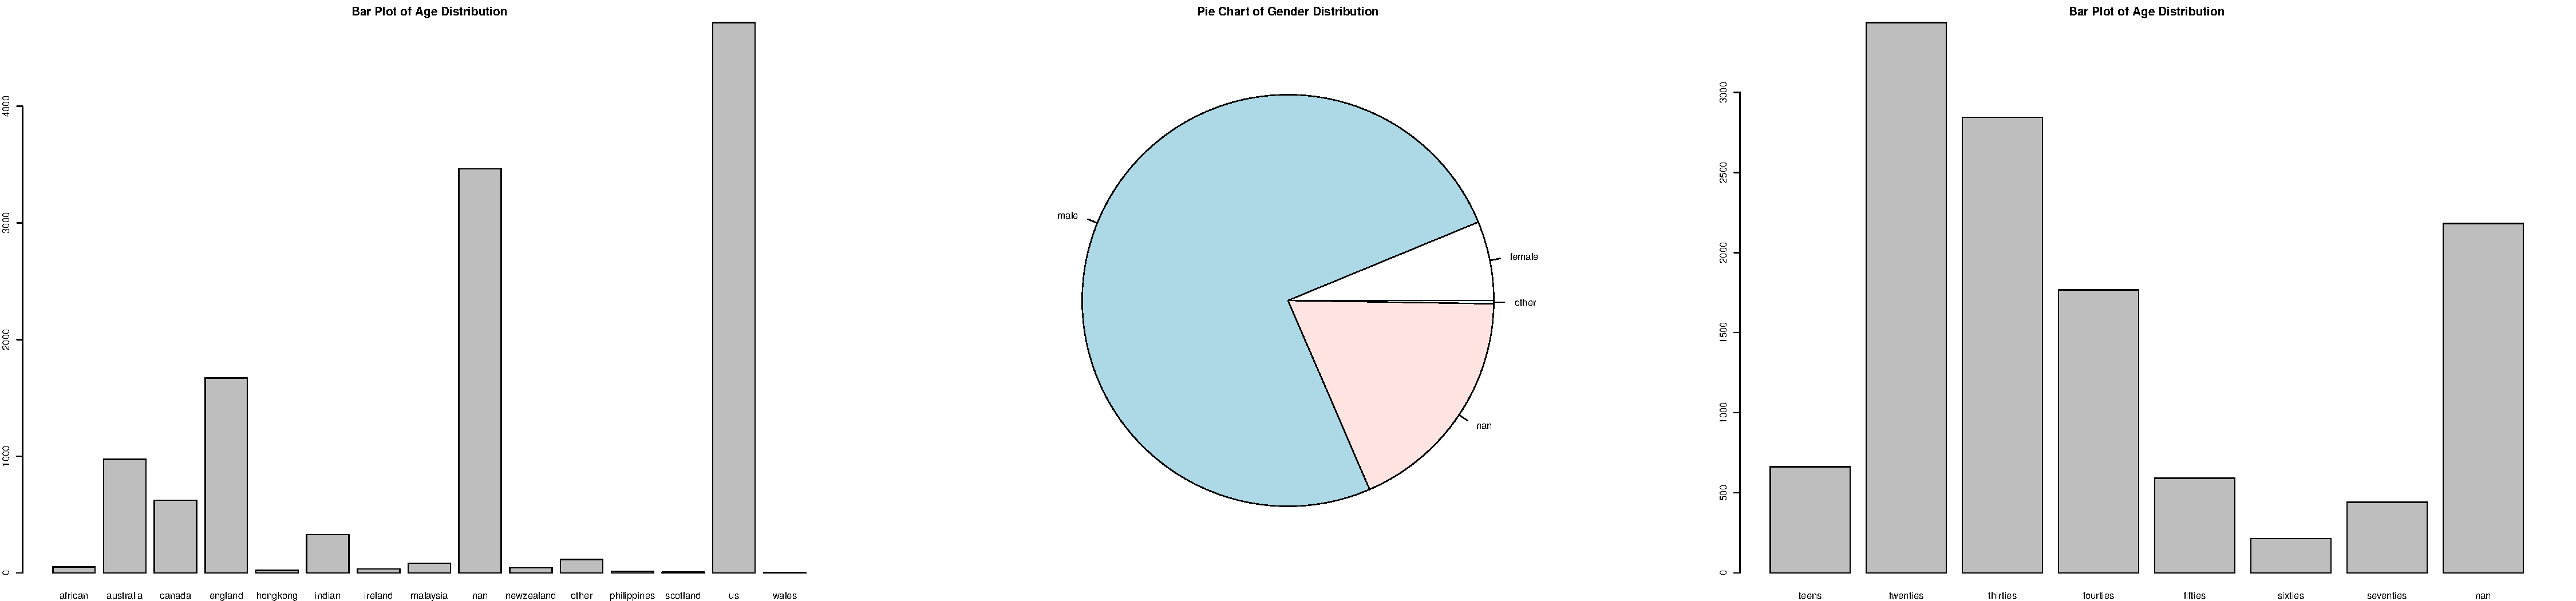
\includegraphics[width=\textwidth]{graphs/distribution.pdf}
		\caption{The distribution of different genders, regional accents, and age groups.}
		\label{distribution}
	\end{figure}
	
	The feature extraction pipeline for voice data involves the following steps:
	\begin{enumerate}
		\item \textbf{Audio Loading}: Initially, raw audio files are loaded and transformed into digital waveforms, serving as the foundation for subsequent analysis.
		\item \textbf{Preprocessing}: The audio waveforms undergo normalisation and resampling procedures to ensure uniformity across the dataset.
		\item \textbf{Feature Extraction}: Subsequently, a comprehensive set of acoustic features is extracted, including Mel-frequency cepstral coefficients (MFCCs), spectral centroid, spectral entropy, spectral flatness, pitch, and magnitude, each providing insights into different facets of the audio signal.
		\item \textbf{Statistical Aggregation}: To synthesize the extracted data, statistical metrics such as the mean, standard deviation, and median are computed, offering a condensed yet informative representation of the features.
	\end{enumerate}
	
	This pipeline transforms raw voice recordings into a set of numerical descriptors that capture the essential qualities of the audio for analytical tasks.
	
	The descriptions of the extracted features have been listed in Table \ref{table:features_description}.
	
	{
		\renewcommand{\arraystretch}{1.3}
		\begin{table}
			\centering
			\begin{tabular}{lll}
				\hline
				\textbf{Feature Name} & \textbf{Feature Description} & \textbf{Feature Type} \\
				\hline
				\texttt{meanfreq} & Average frequency (kHz) & Continuous Variable \\
				\texttt{sd} & Frequency standard deviation & Continuous Variable \\
				\texttt{median} & Median frequency (kHz) & Continuous Variable \\
				\texttt{Q25} & First quartile (kHz) & Continuous Variable \\
				\texttt{Q75} & Third quartile (kHz) & Continuous Variable \\
				\texttt{IQR} & Interquartile range (kHz) & Continuous Variable \\
				\texttt{skew} & Skewness of the frequency distribution & Continuous Variable \\
				\texttt{kurt} & Kurtosis of the frequency distribution & Continuous Variable \\
				\texttt{sp.ent} & Spectral entropy & Continuous Variable \\
				\texttt{sfm} & Spectral flatness measure & Continuous Variable \\
				\texttt{mode} & Mode frequency & Continuous Variable \\
				\texttt{centroid} & Frequency centroid & Continuous Variable \\
				\texttt{meanfun} & Mean fundamental frequency across the signal & Continuous Variable \\
				\texttt{minfun} & Minimum fundamental frequency across the signal & Continuous Variable \\
				\texttt{maxfun} & Maximum fundamental frequency across the signal & Continuous Variable \\
				\texttt{meandom} & Mean dominant frequency across the signal & Continuous Variable \\
				\texttt{mindom} & Minimum dominant frequency across the signal & Continuous Variable \\
				\texttt{maxdom} & Maximum dominant frequency across the signal & Continuous Variable \\
				\texttt{dfrange} & Dominant frequency range & Continuous Variable \\
				\texttt{modindx} & Modulation index & Continuous Variable \\
				\texttt{age} & Age of the speaker & Ordinal Variable \\
				\texttt{gender} & Gender of the speaker & Nominal Variable \\
				\texttt{accent} & Accent of the speaker & Nominal Variable \\
				\hline
			\end{tabular}
			\caption{Description of Features}
			\label{table:features_description}
		\end{table}
	}
	
	For enhanced accessibility, the DiffVoice dataset, along with its comprehensive feature set, has been systematically catalogued into CSV files and the HuggingFace Dataset form~\cite{lhoest2021datasets}, providing a centralized and user-friendly repository for data exploration and analysis. The dataset is available for download at \url{https://huggingface.co/datasets/pufanyi/DiffVoice}.	
	
	\subsection{Data Preparation}
	
	\subsubsection{Data Normalization}
	
	The data preparation process starts with normalizing data, the steps can be described as follows:
	
	\begin{enumerate}
		\item \textbf{Visualizing Data}: Gaining a basic understanding of the data distribution using histogram and boxplot. This visual representation easily allows us to assess the skewness or symmetry of these distributions.
		\item \textbf{Assessing Normality}: We then proceed to assess the normality of data by imposing a normal PDF on the histogram and Quantile-Quantile Plot (QQ-plot).
		\item \textbf{Data Transformation}: If the data is not normal, we tried to transform the data by selecting a proper transformation function, and go to step 2 to check for normality again.
	\end{enumerate}
	
	Fig.~\ref{data_prep} presents the comprehensive pipeline for data normalisation.
	\begin{figure}
		\centering
		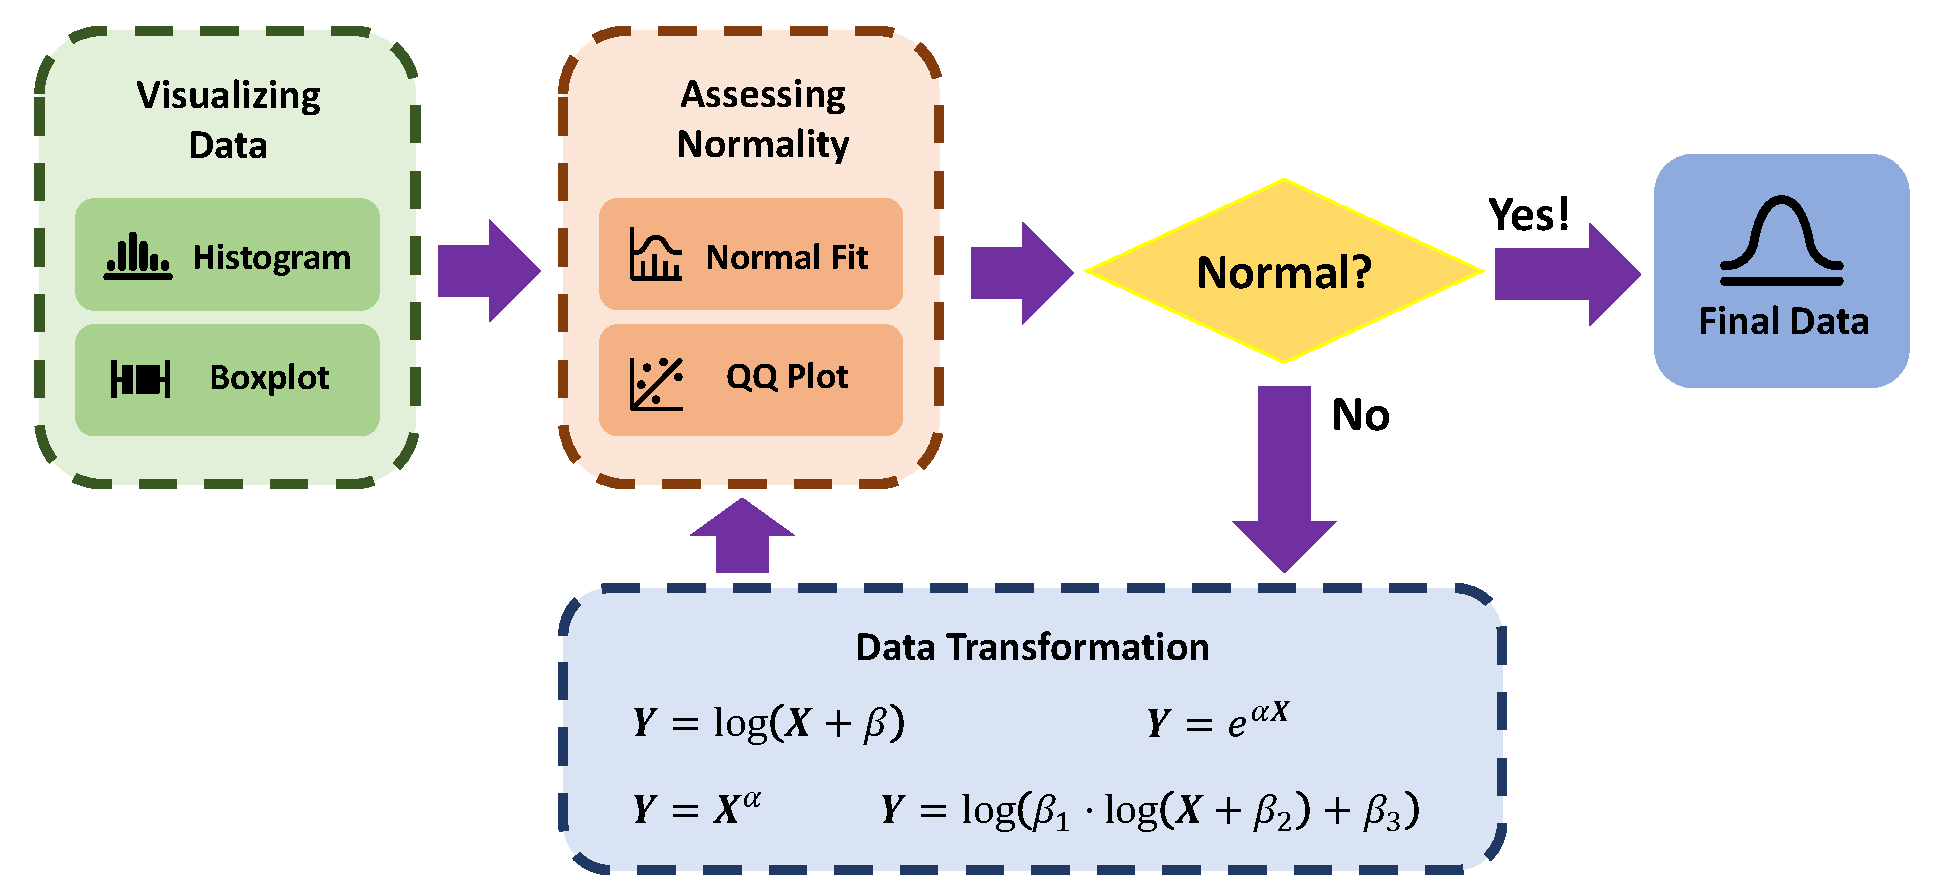
\includegraphics[width=\textwidth]{graphs/prepare_data.pdf}
		\caption{The pipeline for data preparation.}
		\label{data_prep}
	\end{figure}
	
	Table~\ref{tab:feature_transformations} provides a detailed summary of the results from our data preparation phase.
	
	{
		\renewcommand{\arraystretch}{1.5}
		\begin{table}
			\centering
			\begin{tabularx}{\textwidth}{@{}lXlX@{}}
				\toprule
				\textbf{Feature} & \textbf{Before Transformation} & \textbf{Transformation Function} & \textbf{After Transformation} \\
				\midrule
				\texttt{meanfreq} & Almost Normal & $\log(x)$ & Normal \\
				\texttt{sd} & Not Normal & $\log(x + 300)$ & Normal \\
				\texttt{median} & Not Normal & $\log(x + 0.01)$ & Almost \\
				\texttt{Q25} & Not Normal & $\log(x  + 70)$ & Almost \\
				\texttt{Q75} & Not Normal & $\log(x + 5000)$ & Normal \\
				\texttt{IQR} & Almost Normal & - & - \\
				\texttt{skew} & Almost Normal & - & - \\
				\texttt{kurt} & Almost Normal & - & - \\
				\texttt{sp.ent} & Not Normal & $\sqrt{\log(x) + 10}$ & Normal \\
				\texttt{sfm} & Not Normal & $\sqrt{\log(x) + 10}$ & Almost Normal \\
				\texttt{mode} & Almost Normal & $\log(x + 100)$ & Normal \\
				\texttt{centroid} & Not Normal & $\log(x)$ & Normal \\
				\texttt{meanfun} & Not Normal & $\log(x + 3)$ & Almost Normal \\
				\texttt{minfun} & Not Normal & $\log(10 \log(x - 151.35) + 0.7)$ & Almost Normal \\
				\texttt{maxfun} & Not Normal & - & Not Normal \\
				\texttt{meandom} & Not Normal & $\log(x+ 0.01)$ & Almost Normal \\
				\texttt{mindom} & Not Normal & $\log(x)$ & Almost Normal \\
				\texttt{maxdom} & Not Normal & $\sqrt[3]{x}$ & Normal \\
				\texttt{dfrange} & Not Normal & $\sqrt[3]{x}$ & Almost \\
				\texttt{modindx} & Almost Normal & $\sqrt[3]{x}$ & Normal \\
				\bottomrule
			\end{tabularx}
			\caption{Normalization transformations applied to features}
			\label{tab:feature_transformations}
		\end{table}
	}
	
	Histograms are utilized to depict the distribution of variables pre- and post-transformation, as illustrated in Fig.~\ref{transformation_hist}.
	\begin{figure}
		\centering
		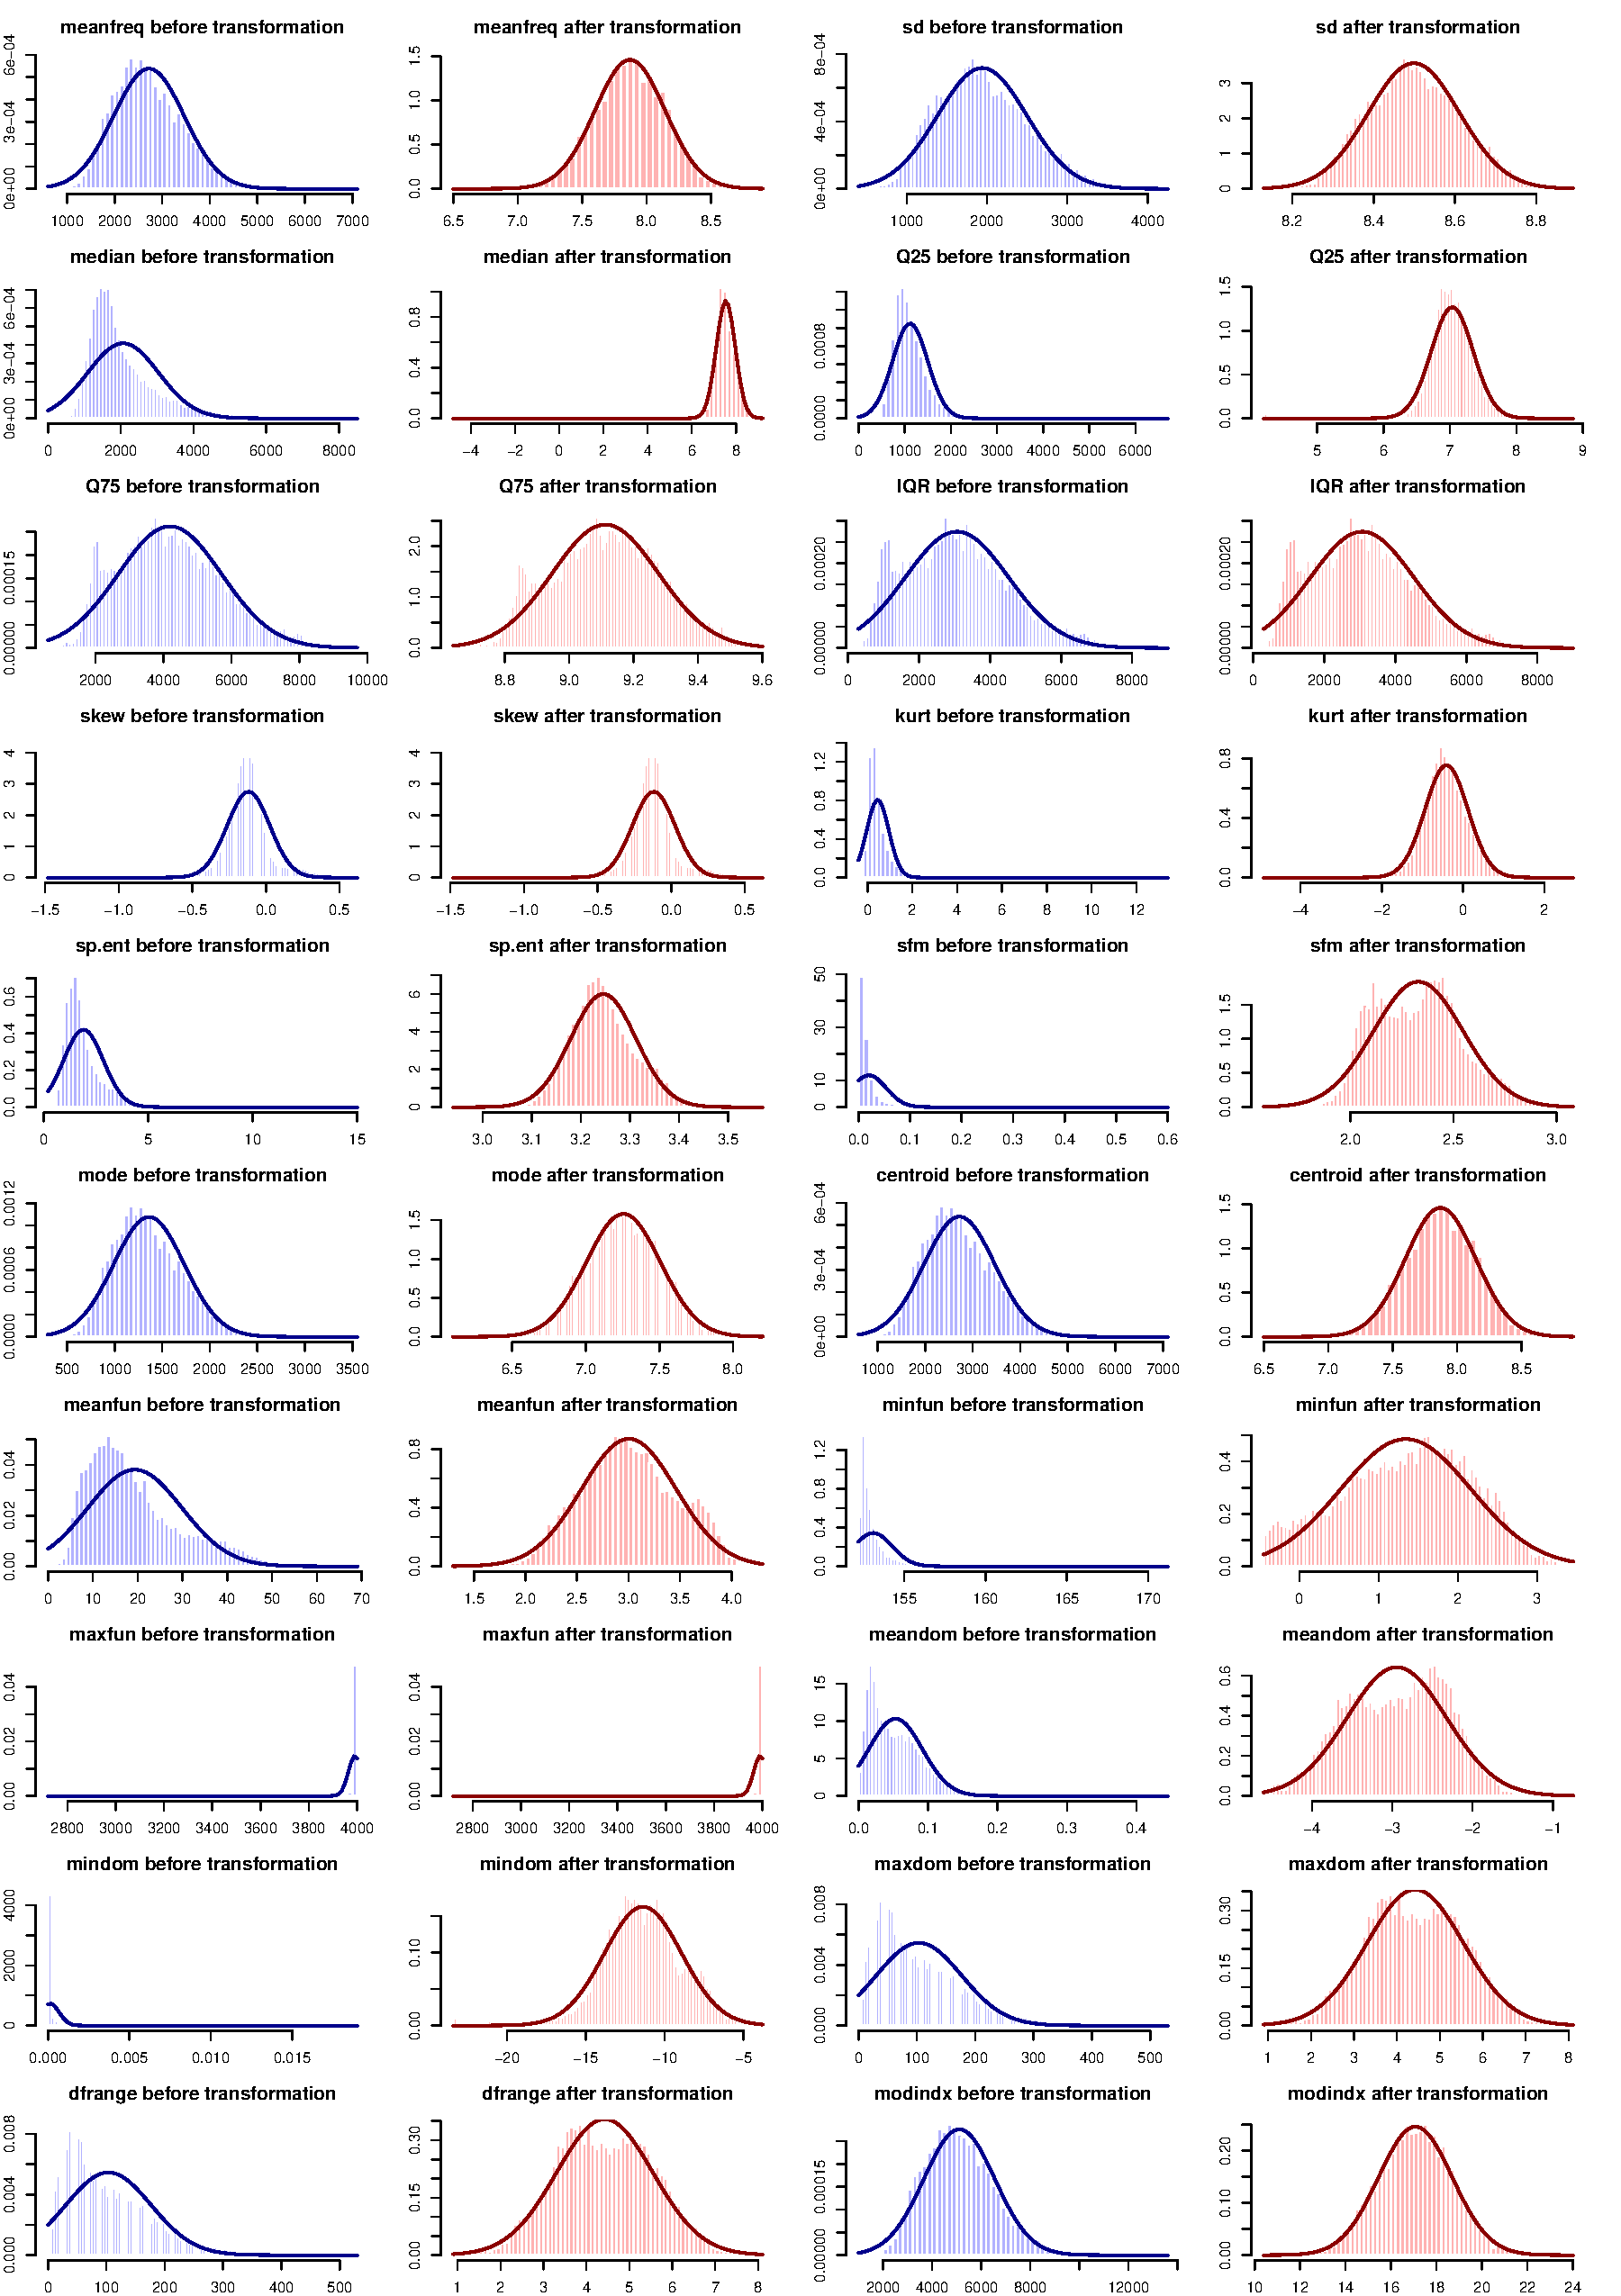
\includegraphics[width=\textwidth]{graphs/transformations_hist.pdf}
		\caption{Histogram of variables before and after transformation.}
		\label{transformation_hist}
	\end{figure}
	
	Additionally, QQ-plots are employed to assess the normality of the variables, with comparisons drawn between their states before and after transformation, as shown in Fig.~\ref{transformation_qq}.
	\begin{figure}
		\centering
		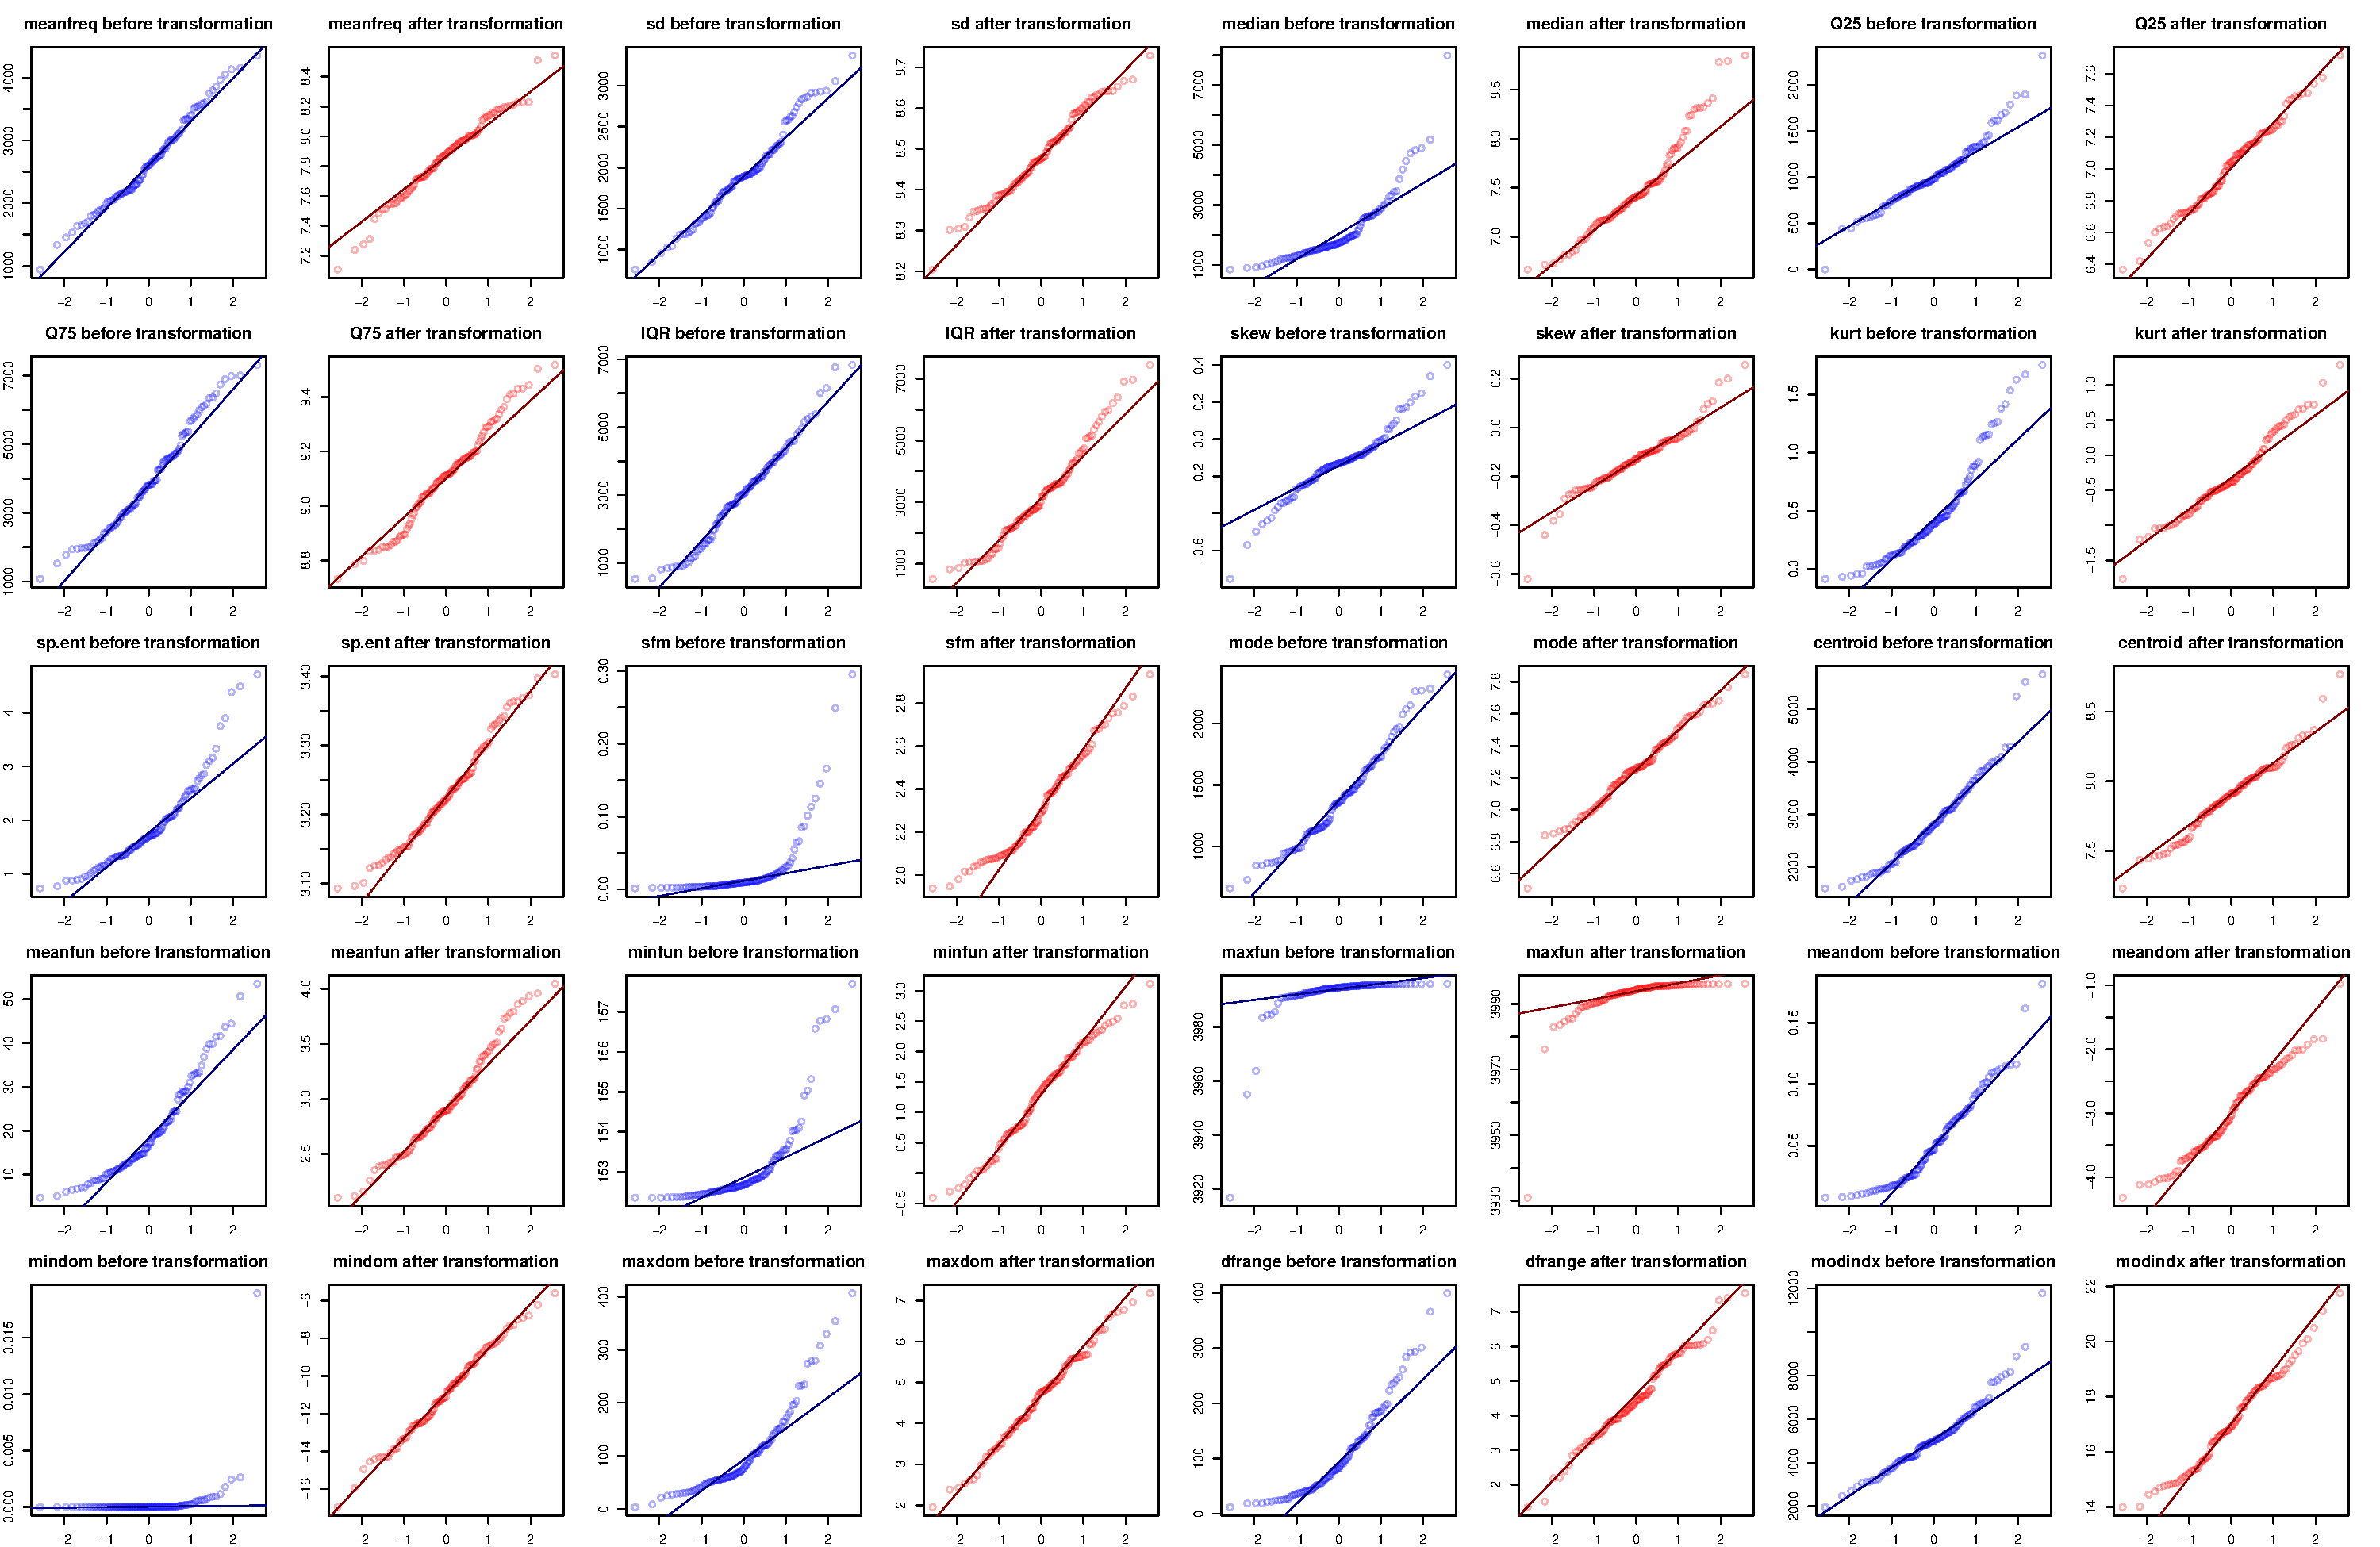
\includegraphics[width=\textwidth]{graphs/transformations_qq.pdf}
		\caption{QQ-plot of variables before and after transformation.}
		\label{transformation_qq}
	\end{figure}
	
	For an illustration of the code used to normalize the \texttt{sd} column, see Appendix~\ref{appendix:data_trans}.	
	
	\subsubsection{Feature Selection}
	
	After transformation, we selected 9 features for further analysis: \texttt{meanfreq}, \texttt{sd}, \texttt{median}, \texttt{Q25}, \texttt{Q75}, \texttt{skew}, \texttt{sp.ent}, \texttt{sfm}, \texttt{meanfun}.
	
	\subsubsection{Balancing Data}
	
	An initial data review revealed a significant imbalance, with male voice samples outnumbering female ones, as depicted in Fig.~\ref{distribution}. The presence of entries with unspecified gender further complicated the analysis.
	
	To address this, we equalized the gender distribution within the dataset, ensuring that female data were not overshadowed or misclassified as anomalies. We randomly selected samples from the predominant gender category until they matched the count of the less-represented gender.
	
	\subsubsection{Outlier Removal}
	
	Following the balancing of the dataset, we conducted a thorough examination to detect outliers, as such will enable us to maintain an equitable and impartial representation of both genders. Outliers were defined as observations with values exceeding 1.5 times the interquartile range (IQR), which is the range between the first and third quartiles. This method helps identify and address data points that are significantly different from the overall pattern, ensuring the integrity of our analysis.
	
	\subsubsection{Rebalancing Data}
	
	Finally, we rebalance the data to ensure gender equality.
	
	After all the preparation, there are a total of 1444 observations from female and male samples, with 722 male samples and 722 female samples.
	
	\section{Data Analysis and Testing}
	
	\subsection{Data Analysis By Gender}
	
	\subsubsection{General Description}
	
	The analysis methods generally unfold through the following stages:
	
	\begin{itemize}
		\item \textbf{Data Visualization}: We begin by creating a histogram and a boxplot to visually inspect the distribution of the data, seperated by gender, shown in Fig.~\ref{hist_bothgender}.
		\item \textbf{Assessing Normality}: Next, we check the normality by different methods including the graph overlaid with a normal pdf, QQ-plot (Fig.~\ref{qq_male} for male and Fig.~\ref{qq_female} female) and Shapiro-Wilk test~\cite{shapiro1965analysis}.
	\end{itemize}
	If the data is normally distributed, we conduct an F-test to compare the variance of the data.
	\begin{itemize}
		\item Comparing variance using \textbf{F-test}: If the p-value from the F-test is less than 0.05, we reject the null hypothesis that the variance of the data is the same across groups. Otherwise, we do not reject the null hypothesis.
		\item Using \textbf{two sample t-test}: We proceed to perform a two-sample t-test. If the p-value from the t-test is less than 0.05, we reject the null hypothesis that the mean of the data is the same across groups. Otherwise, we do not reject the null hypothesis.
	\end{itemize}
	If the data is not normally distributed, we employ the Wilcoxon test to compare the mean of the data.
	\begin{itemize}
		\item \textbf{Wilcoxon test} for non-normally distributed data: If the p-value from the Wilcoxon test is less than 0.05, we reject the null hypothesis that the mean of the data is the same across groups. Additionally, by specifying the side in the Wilcoxon test, we can determine which group has a smaller mean.
	\end{itemize}
	\begin{figure}
		\centering
		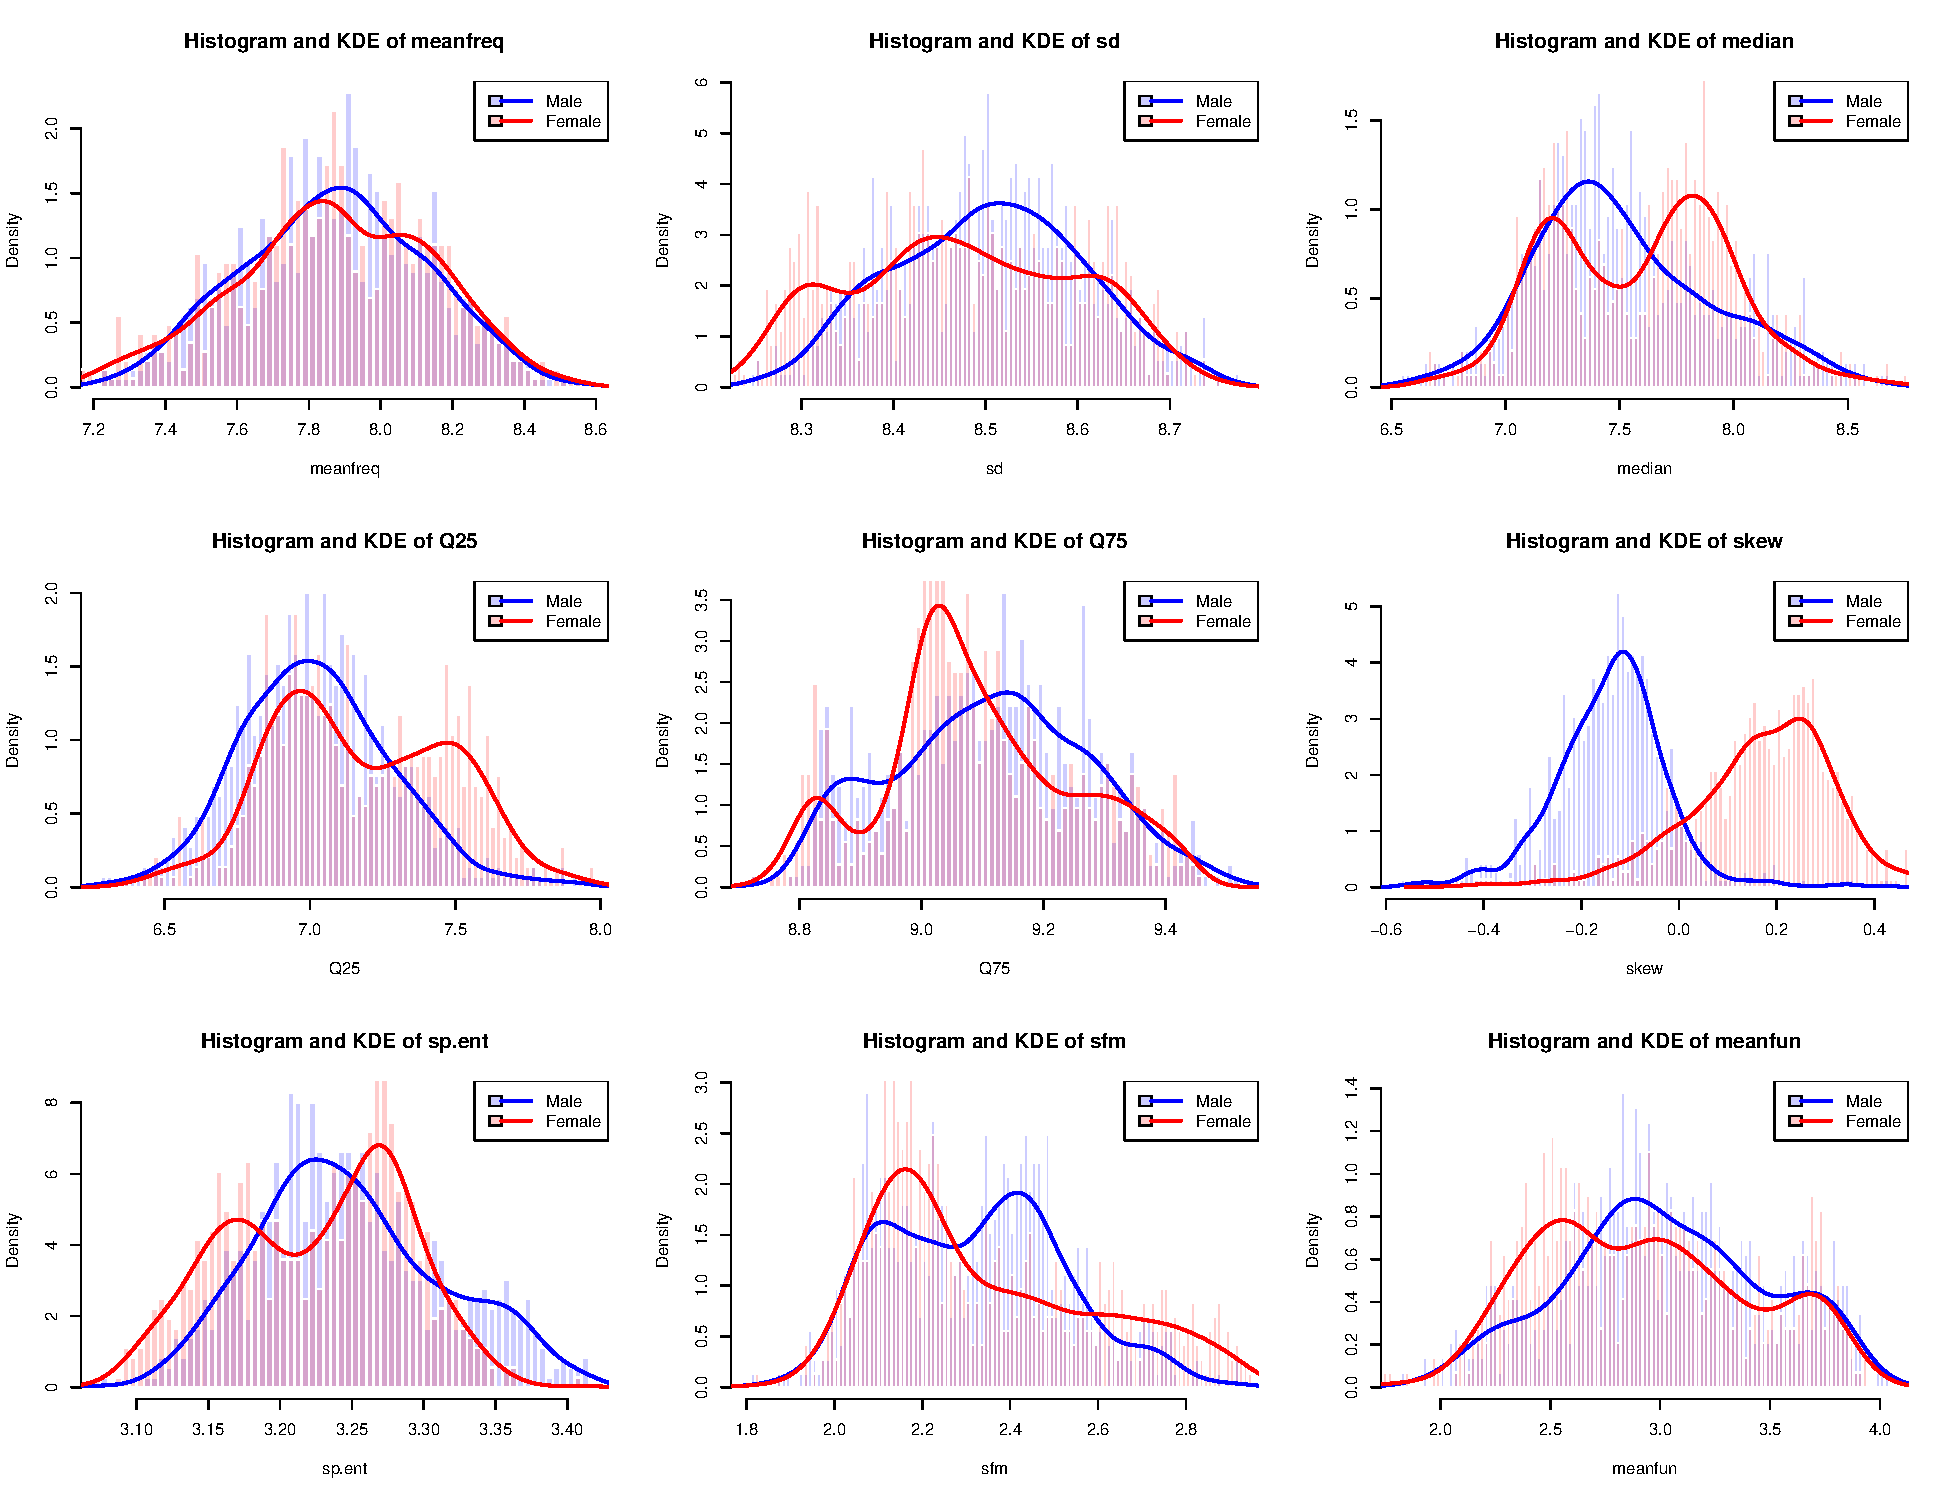
\includegraphics[width=\textwidth]{graphs/gender/visualizations.pdf}
		\caption{Histogram of variables in both genders.}
		\label{hist_bothgender}
	\end{figure}
	\begin{figure}
		\centering
		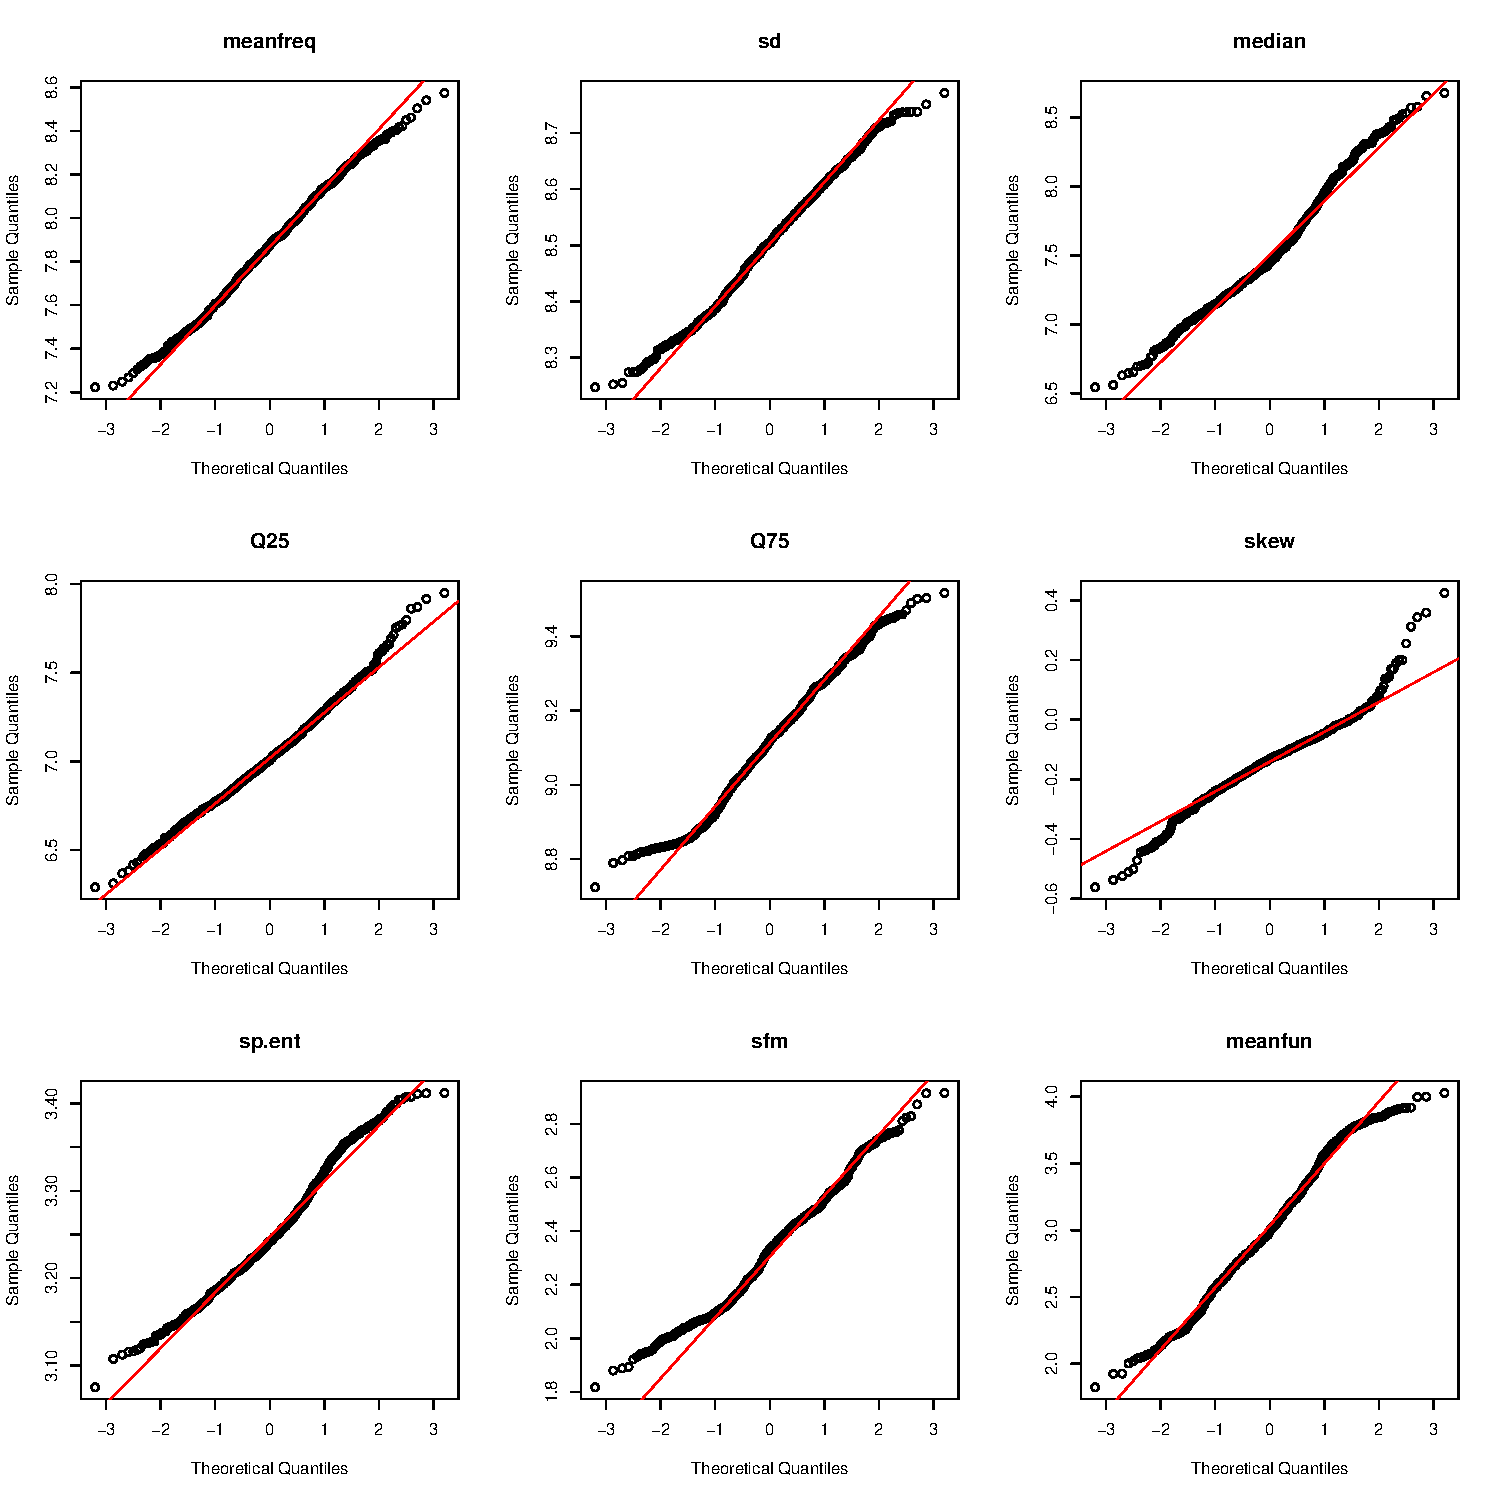
\includegraphics[width=\textwidth]{graphs/gender/qq_plot_male.pdf}
		\caption{QQ-plot of male dataset.}
		\label{qq_male}
	\end{figure}
	\begin{figure}
		\centering
		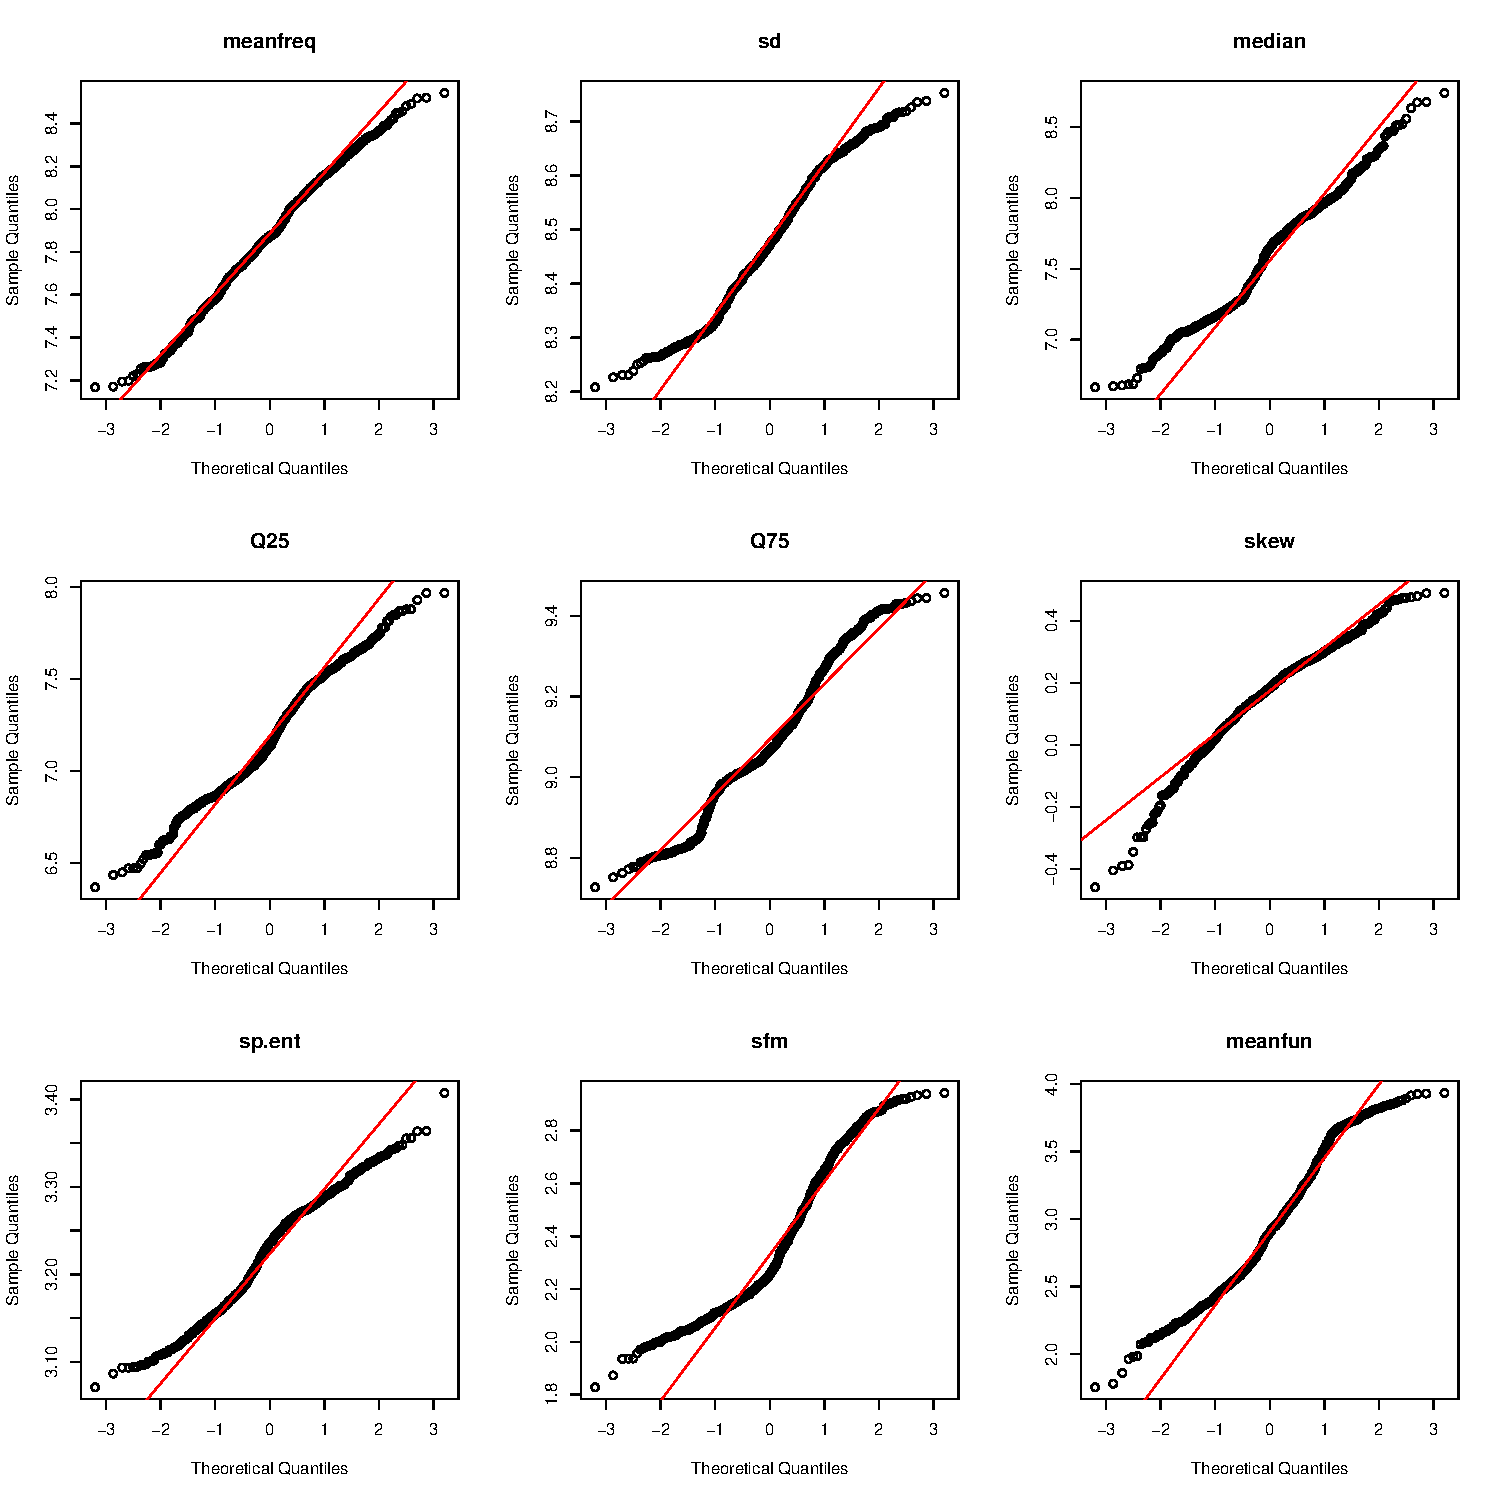
\includegraphics[width=\textwidth]{graphs/gender/qq_plot_female.pdf}
		\caption{QQ-plot of female dataset.}
		\label{qq_female}
	\end{figure}
	
	\subsubsection{Analysis in Different Features}
	
	\textbf{Mean Frequency} Regarding \texttt{meanfreq}, we observe that the data for both males and females are normally distributed. Consequently, we first apply an F-test to evaluate whether the variances for male and female data are equivalent. With the null hypothesis $H_0$: \textit{males and females have the same variance} and the alternative hypothesis $H_1$: \textit{males and females have different variances}, we obtain a p-value of $0.04445$. This result leads us to reject $H_0$ in favour of $H_1$. Subsequently, we conduct a t-test with $H_0$: \textit{males and females have the same means} against $H_1$: \textit{males and females have different means}. The resulting p-value of $0.849$ indicates that we cannot reject $H_0$. Contrary to intuition, this suggests that there is virtually no difference in mean frequency between males and females. Then, what could be the cause behind the common perception that female voices are more shrill than male voices? We attempt to investigate this further by examining other variables.
	
	\textbf{Median Frequency} The non-parametric test -- one-sided Wilcoxon Test is applied due to the non-normal distribution, with null hypothesis $H_0$: \textit{Distribution of male \texttt{median} and female \texttt{median} are the same}; alternative hypothesis $H_1$: \textit{Distribution of male \texttt{median} has smaller values than female \texttt{median}}. The p-value from the test is $8.022\times 10^{-5}$ which is less than the significant value. Thus, we reject $H_0$ in favour of $H_1$, supporting the distribution of male \texttt{median} has smaller values than female \texttt{median}. This indicates that males generally have a lower median pitch in their voices compared to females.
	
	\textbf{First Quartile of Frequency} While the \texttt{Q25} data for males is normally distributed, the skewness observed in the female \texttt{Q25} necessitates the use of a non-parametric test. We employ a one-sided Wilcoxon test, positing the null hypothesis $H_0$: \textit{The distributions of male and female \texttt{Q25} are identical}, against the alternative hypothesis $H_1$: \textit{The distribution of male \texttt{Q25} skews towards smaller values compared to female \texttt{Q25}.} The exceedingly small p-value of $2.2\times 10^{-16}$, well below the threshold of significance, leads us to reject $H_0$ in favor of $H_1$. This finding corroborates that the distribution of male \texttt{Q25} indeed gravitates towards smaller values than that of females. This suggests that despite similar average frequencies, females tend to have fewer low-frequency components in their voices compared to males.
	
	\textbf{Third Quartile of the Frequency} After justifying the non-normal distribution of the data, a one-sided Wilcoxon test is applied, with null hypothesis $H_0$: \textit{Distribution of male \texttt{Q75} and female \texttt{Q75} are the same}; alternative hypothesis $H_1$: \textit{Distribution of male \texttt{Q75} has smaller values than female \texttt{Q75}}. The p-value from the test is $0.0007$ which is less than the significant value. Thus, we reject $H_0$ in favour of $H_1$, supporting the distribution of male \texttt{Q75} has greater values than female \texttt{Q75}. This is also quite surprising, which means that in fact, males are capable of producing high-pitched sounds as well.
	
	\textbf{Skewness of the Frequency Distribution} Same as above, a one-sided Wilcoxon test is applied, with null hypothesis $H_0$: \textit{Distribution of male \texttt{skew} and female \texttt{skew} are the same}; alternative hypothesis $H_1$: \textit{Distribution of male \texttt{skew} has smaller values than female \texttt{skew}}. The p-value from the test is $2.2\times 10^{-16}$ which is less than the significant value. Thus, we reject $H_0$ in favour of $H_1$, supporting the distribution of male \texttt{skew} has smaller values than female \texttt{skew}. Another interesting thing we can find in Fig~\ref{hist_bothgender} is that most of the females are right-skew and most of the males are left-skew. This could suggest that male voices tend to have a fuller sound in the lower frequency range, while female voices may exhibit a fuller sound in the higher frequency range.
	
	
	\textbf{Spectral Entropy} One-sided Wilcoxon test is applied, with null hypothesis $H_0$: \textit{Distribution of male \texttt{sp.ent} and female \texttt{sp.ent} are the same}; alternative hypothesis $H_1$: \textit{Distribution of male \texttt{sp.ent} has smaller values than female \texttt{sp.ent}}. The p-value from the test is $5.564\times 10^{-8}$ which is less than the significant value. Thus, we reject $H_0$ in favour of $H_1$, supporting the distribution of male \texttt{sp.ent} has larger values than female \texttt{sp.ent}. Which suggests that there is a greater complexity or randomness in their sound spectra. This could imply that male voices have a richer variety of frequencies or a less predictable structure compared to female voices, potentially contributing to a perception of a ``rougher'' or more ``textured'' quality in male speech. 
	
	\textbf{Spectral Flatness Measure} In this case, a two-sided Wilcoxon test is applied, with null hypothesis $H_0$: \textit{Distribution of male \texttt{sfm} and female \texttt{sfm} have no significant difference}; alternative hypothesis $H_1$: \textit{Distribution of male \texttt{sfm} has significant difference compared female \texttt{sfm}}. The p-value from the test is $0.8317$ which is larger than the significant value. Thus, we do not reject $H_0$ in favour of $H_1$, supporting the distribution of male \texttt{sfm} has no significant difference compared to female \texttt{sfm}.
	
	\textbf{Mean Fundamental Frequency Across the Signal} The data in \texttt{meanfun} are not normally distributed as suggested from the result of the Shapiro-Wilk Test, we apply the non-parametric test -- Wilcoxon Test with null hypothesis $H_0$: \textit{Distribution of male \texttt{meanfun} and female \texttt{meanfun} are the same}; alternative hypothesis $H_1$: \textit{Distribution of male meanfun has larger values than female \texttt{meanfun}}. The p-value from the test is $1.859\times 10^{-5}$ which is less than the significant value. Thus, we reject H0 in favor of H1, supporting the distribution of male \texttt{meanfun} has higher values than female \texttt{meanfun}.
	
	
	% 要不不删了就留在这里当纪念吧
	%%%%%%%%%%%%%%%%%%%%%%%%%%%%% 以下是一座纪念碑 %%%%%%%%%%%%%%%%%%%%
	% 你俩怎么都在这儿                                                %
	% 我很慌regression                                              %
	% 我感觉其他的都稍微ok点了我要不                                    %
	% 还有四小时                                                     %
	% 啊啊啊啊啊啊啊啊啊啊啊啊啊糟糕了                                   %
	% 呜呜呜                                                        %
	% 没关系!                                                       %
	% 我九点钟就去搞regression                                        %
	% okok                                                          %
	% 三个小时肯定能行!
	% 加油加油呜呜呜
	% 糟糕我太拖延了
	% 啊啊啊啊啊啊啊啊啊啊啊啊啊啊啊赶紧写赶紧写呜呜呜呜
	% 我也是5555555
	% 完蛋嗯嗯嗯嗯
	% 芭比q
	% 不行我过会儿再画  越急越爽哈哈哈哈哈哈哈
	% 这个交之后再画了  哈哈哈哈哈哈哈哈
	
	\subsubsection{Outcomes}
	
	The outcomes of our analysis challenge traditional assumptions. We found that, contrary to popular opinion, the average frequencies produced by both male and female voices are nearly identical. Nonetheless, female voices are more commonly found at higher frequency ranges, whereas male voices predominantly occupy lower frequency ranges, even though they are also capable of reaching higher pitches. Moreover, the sound spectra of male voices demonstrate a higher degree of complexity or variability, potentially leading to the impression that male voices have a ``rougher'' or more ``textured'' quality.	
	
	\subsection{Data Analysis By Age}
	We investigate whether distinct age groups exhibit varying characteristics. This examination utilizes the same features as those employed in the gender analysis.
	
	\subsubsection{Methodology}
	Similar to the approaches in analysis of gender, we balance the data based on gender equity first. Then we conduct the following step on each features across different age groups:
	\begin{itemize}
		\item Visualizing the data: \textbf{Boxplots} are firstly used to illustrate the distribution of the data across different age groups. Each boxplot displays the median, quantiles, and outliers for each age group.
		\item Checking for normality: \textbf{Shapiro-Wilk tests} are performed on the mean frequency data within each age group to determine if the data follows a normal distribution.
		\item Comparing differences between age groups:
		\begin{itemize}
			\item For normally distributed data, we employ an \textbf{ANOVA} model to discern any significant differences across age groups.
			\item For data that does not follow a normal distribution, \textbf{Kruskal-Wallis tests} are utilized to identify significant differences between age groups.
		\end{itemize}
		\item Upon detecting notable differences, we proceed with pairwise comparisons to pinpoint specific age groups that differ:
		\begin{itemize}
			\item \textbf{Pairwise t-tests} are used for data adhering to normality.
			\item For non-normal data, \textbf{pairwise Wilcoxon tests} are conducted.
		\end{itemize}
	\end{itemize}
	
	We would now use the test for mean frequency across different age groups as an example. We first visualise the distribution of the data in Fig.~\ref{meanfreq_age}
	\begin{figure}
		\centering
		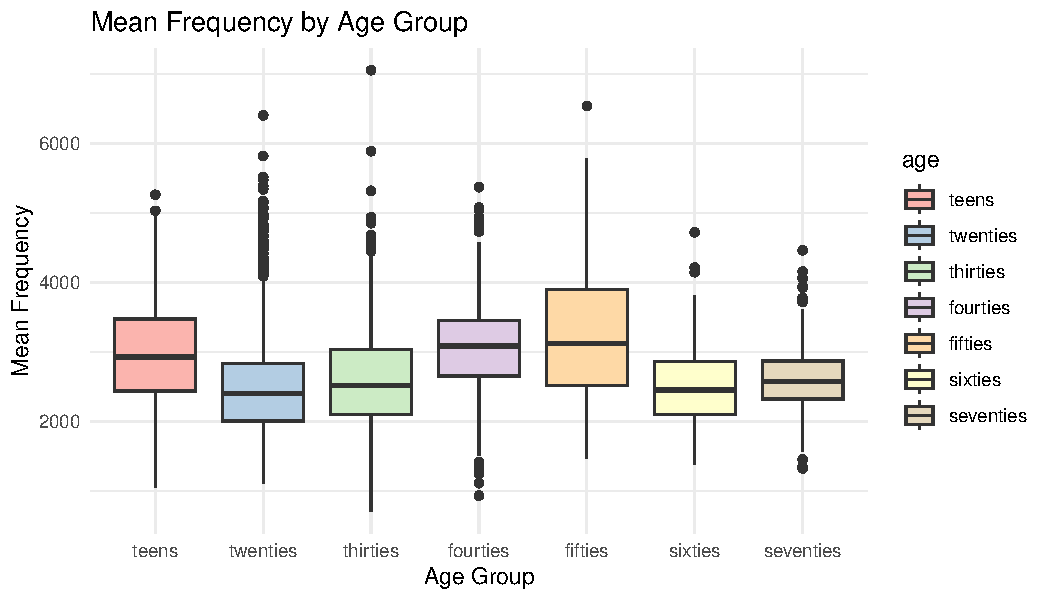
\includegraphics[width=\textwidth]{graphs/age/mean_frequency_by_age_group.pdf}
		\caption{Mean Frequency by Age Group.}
		\label{meanfreq_age}
	\end{figure}
	The Shapiro-Wilk test suggest that most age group does not follow a normal distribution. The result of the Pairwise Wilcoxon Test is shown in Fig.~\ref{meanfreq_age_result}
	\begin{figure}
		\centering
		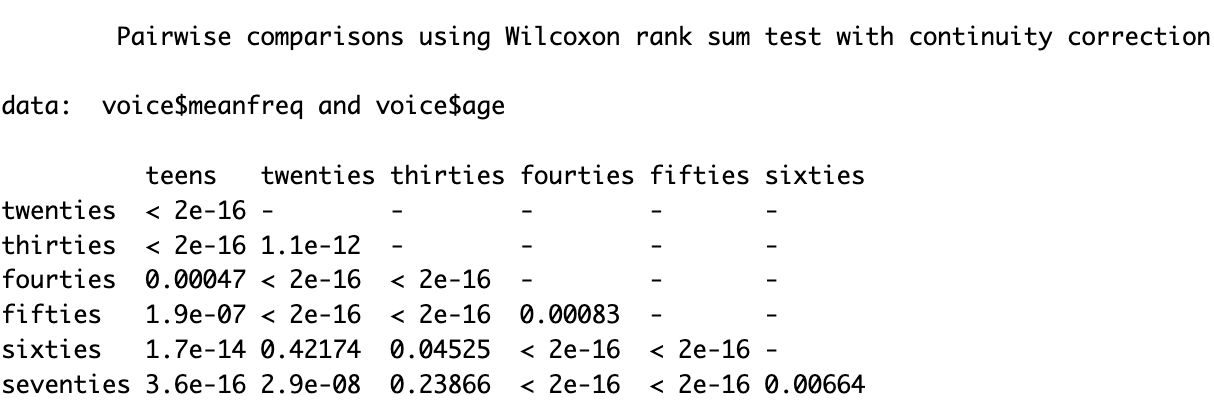
\includegraphics[width=\textwidth]{graphs/age/meanfreq_result.png}
		\caption{Pairwise Wilcoxon Test Result.}
		\label{meanfreq_age_result}
	\end{figure}
	
	We perform tests for each feature. For each feature, data is not normally distributed based on the age group, and the result of Shapiro-Wilk test suggests that there is no feature such that there is no significance difference between all age groups. there and the detailed results will be provided in the appendix.
	\subsubsection{Outcomes}
	
	After the tests, we listed our outcomes as below.
	
	\textbf{meanfreq} There is no significant difference between the mean frequency of the thirties and sixties age groups, nor between the thirties and seventies age groups.
	
	\textbf{sd} There is no significant difference between the standard deviation of the teens and fifties age groups, teens and seventies age groups, thirties and sixties age groups, nor fifties and seventies age groups.
	
	\textbf{Q25} There is no significant difference between the Q25 of the teens, twenties and thirties age groups.
	
	\textbf{Q75} There is no significant difference between the Q75 of the teens and fifties age groups, thirties and sixties age groups, forties and fifties age groups, nor sixties and seventies age groups.
	
	\textbf{skew} There is no significant difference between the skewness of the teens, twenties and sixties age groups, thirties and fifties age groups, nor thirties and sixties age groups.
	
	\textbf{sp.ent} There is no significant difference between the sp.ent of the twenties and sixties age groups.
	
	\textbf{sfm} There is no significant difference between the sfm of the teens and fourties age groups, teens and fifties age groups, twenties and sixties age groups, thirties and seventies, nor sixties and seventies age groups.
	
	\textbf{minfun} There is no significant difference between the minfun of the sixties and seventies age groups.	
	
	\subsection{Correlation Between Numerical Features}
	
	We visualise the correlation between all variables based on the transformed data in Fig.~\ref{correlation_matrix}. We can get a glimpse of the correlation between variables.
	
	\begin{figure}
		\centering
		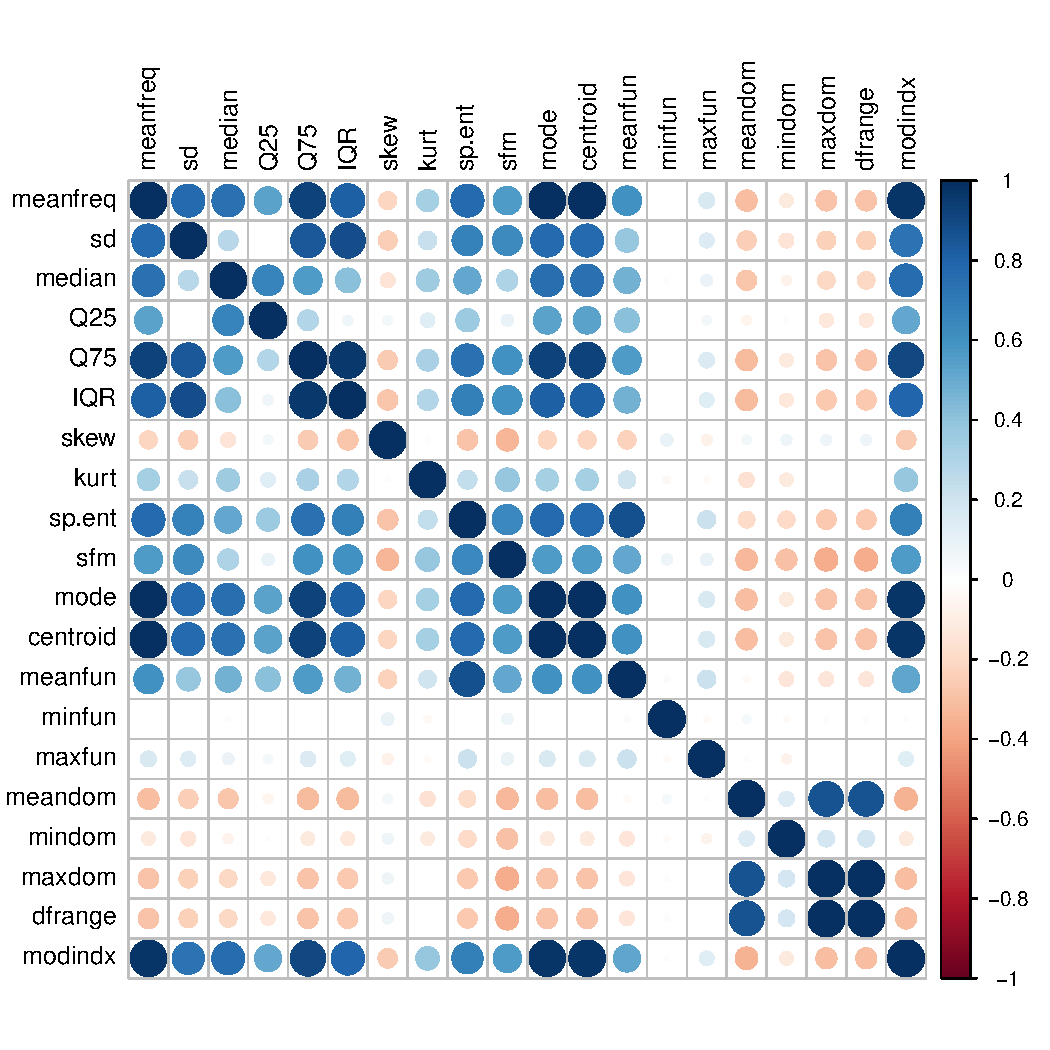
\includegraphics[width=\textwidth]{graphs/correlation_matrix.pdf}
		\caption{Correlation Matrix.}
		\label{correlation_matrix}
	\end{figure}
	
	We also plot a scatter plot to visualize the correlation between some variables (\texttt{meanfreq}, \texttt{median}, \texttt{Q25}, \texttt{Q75}, \texttt{meandom}) based on different genders. As shown in Fig.~\ref{scatter_matrix}.
	\begin{figure}
		\centering
		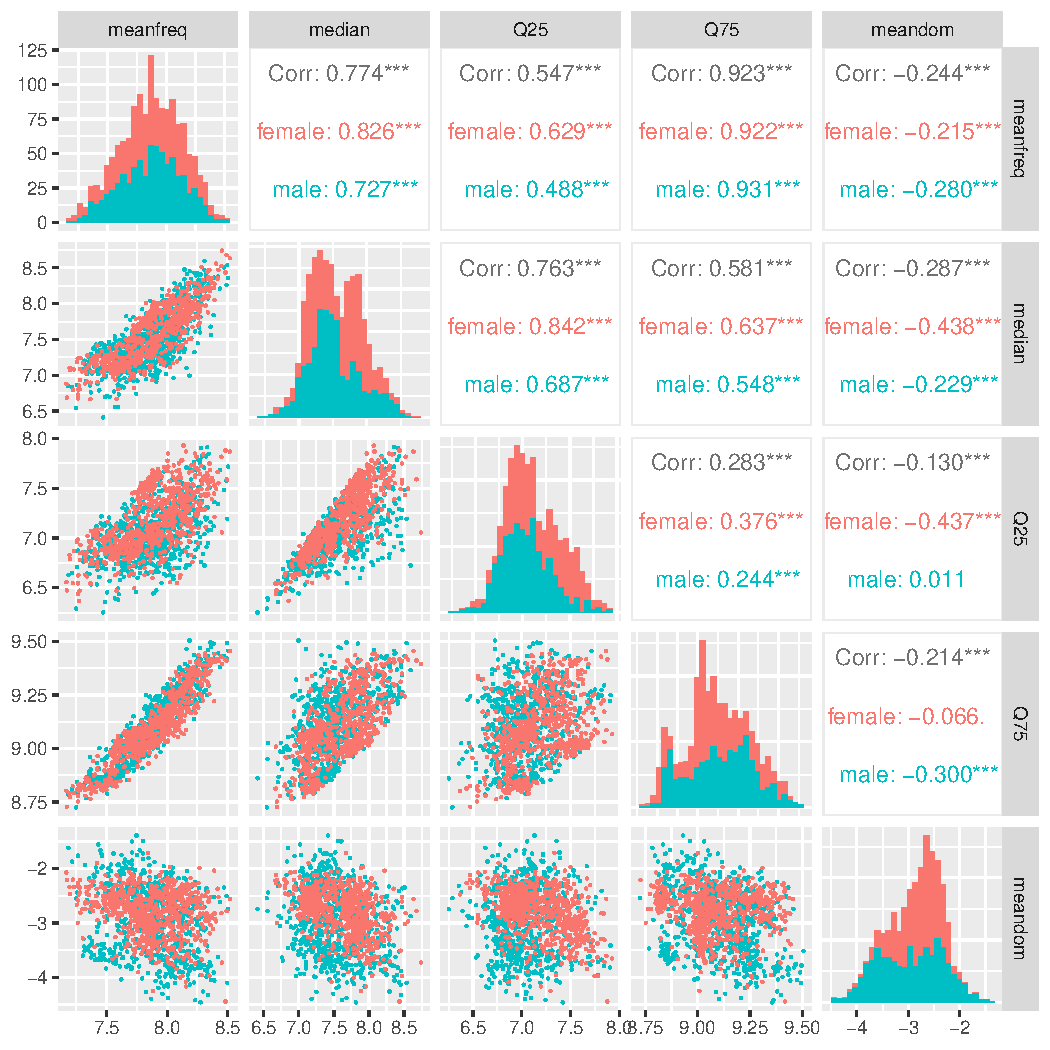
\includegraphics[width=\textwidth]{graphs/scatter_matrix.pdf}
		\caption{Scatter Matrix.}
		\label{scatter_matrix}
	\end{figure}
	
	\section{Regression Analysis}
	
	In this section, we will explore regression analysis techniques to understand the relationship between various features extracted from voice samples and the target variable. Additionally, we will delve into logistic regression and k-nearest neighbours (KNN) classification to predict gender based on voice features.
	
	\subsection{Relations Amount Features of Voice}
	
	\subsubsection{Simple Linear Regression}
	We will begin by examining the relationship between individual features and mean frequency (meanfreq) using simple linear regression. Specifically, we will select a subset of features that are likely to have a significant impact on mean frequency based on prior knowledge or domain expertise. Features such as \texttt{meanfun}, \texttt{meandom}, \texttt{mindom} and \texttt{maxdom} are some of the variables we will consider.
	
	Initially, we perform a correlation test to examine the presence of any relationships. If a non-zero correlation is established, we proceed with linear regression to analyze the relationship between \texttt{meanfreq} and the chosen feature. Finally, we plot a scatter diagram to visualize and assess the efficacy of the model.
	
	\textbf{meanfun} We conduct a correlation test between \texttt{meanfreq} and \texttt{meanfun}, since the p-value is smaller than 0.05, we reject $H_0$. Therefore, the correlation is not equal to 0. We then use simple linear regression model to fit the data, with $\hat{y}=0.30272\cdot x + 6.97028$ and R-Sqaure of 0.2849. Thus, we can conclude that \texttt{meanfreq} and \texttt{meanfun} are positively correlated.
	
	\textbf{meandom} We conduct a correlation test between \texttt{meanfreq} and \texttt{meandom}, since the p-value is smaller than 0.05, we reject $H_0$. Therefore, the correlation is not equal to 0. We then use simple linear regression model to fit the data, with $\hat{y}=-0.12007\cdot x + 7.52414$ and R-Square of 0.2555. Thus, we can conclude that \texttt{meanfreq} and \texttt{meandom} are negatively correlated.
	
	
	\textbf{mindom} We conduct a correlation test between \texttt{meanfreq} and \texttt{mindom}, since the p-value is smaller than 0.05, we reject H0. Therefore, the correlation is not equal to 0. We then use simple linear regression model to fit the data, with $\hat{y}=-0.028755\cdot x + 7.543237$ and R-Sqaure of 0.05978. Thus, we can conclude that \texttt{meanfreq} and \texttt{mindom} are negatively correlated.
	
	\textbf{maxdom} We conduct a correlation test between \texttt{meanfreq} and \texttt{maxdom}, since the p-value is smaller than 0.05, we reject H0. Therefore, the correlation is not equal to 0. We then use simple linear regression model to fit the data, with with $\hat{y}=-0.036590\cdot x + 8.040413$ and R-Square of 0.02178. Thus, we can conclude that \texttt{meanfreq} and \texttt{maxdom} are negatively correlated.
	
	We plotted scatter plot with fitted line for these four features in Fig.~\ref{simple_lr}.
	\begin{figure}
		\centering
		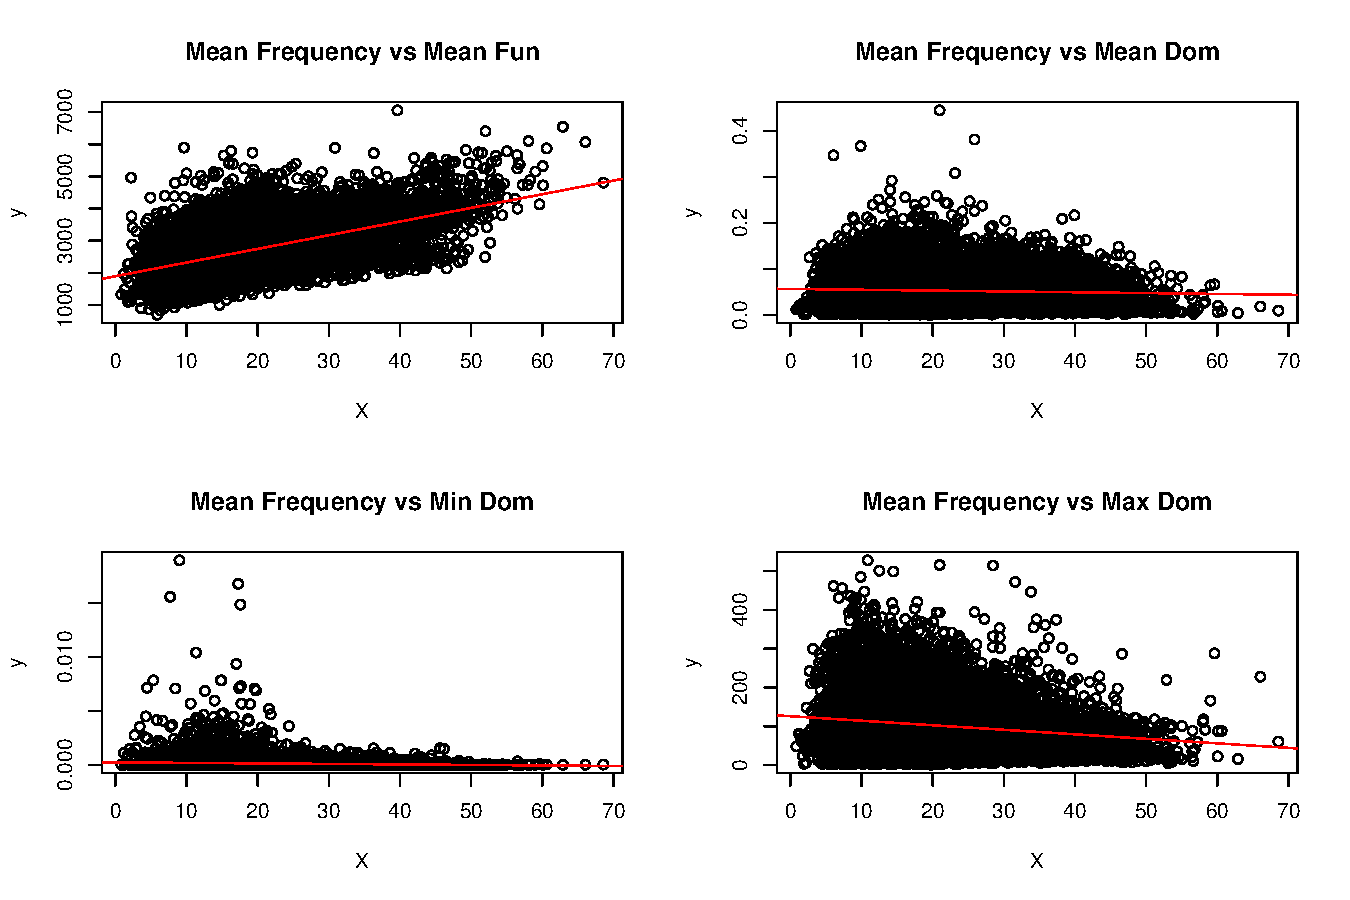
\includegraphics[width=\textwidth]{graphs/simple_linear_regression_plot.pdf}
		\caption{Simple Linear Regression.}
		\label{simple_lr}
	\end{figure}
	
	
	\subsubsection{Multiple Linear Regression}
	
	Moreover, we will extend our analysis to multiple linear regression, where we simultaneously consider multiple predictor variables to predict mean frequency. This will allow us to assess the combined effect of various features on mean frequency, providing a more comprehensive understanding of the relationship. Similar to simple linear regression, we use features such as \texttt{meanfun}, \texttt{meandom}, \texttt{mindom} and \texttt{maxdom} to predict the \texttt{meanfreq}.
	\begin{align*}
		\hat{y}&=2124.7260 \\&+ 43.0794\cdot X_{\text{meanfun}} \\&-7431.3557\cdot X_{\text{meandom}} \\&- 8434.6393\cdot X_{\text{mindom}} \\&+ 1.5605\cdot X_{\text{maxdom}} \\&+ \epsilon
	\end{align*}
	We utilize this formula to predict the value of \texttt{meanfreq}, and generate a diagram as below, Fig.~\ref{multiple_lr}.
	\begin{figure}
		\centering
		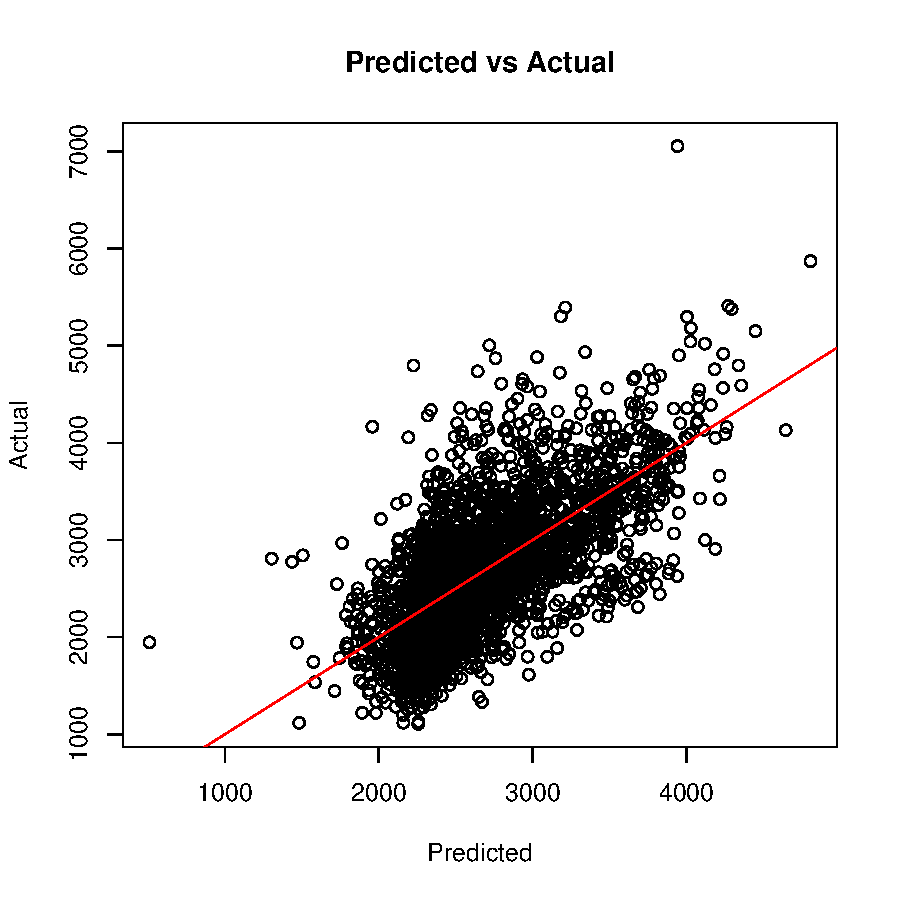
\includegraphics[width=0.5\textwidth]{graphs/multiple_lr.pdf}
		\caption{Multiple Linear Regression.}
		\label{multiple_lr}
	\end{figure}
	
	\subsection{Relationship Between Voice Feature And Speaker}
	
	\subsubsection{Logistic Regression}
	
	Moving beyond linear regression, we will explore logistic regression to predict gender based on voice features. Logistic regression is a powerful tool for binary classification problems, such as predicting gender (male/female) based on voice characteristics. By employing logistic regression, we aim to build a robust predictive model that accurately classifies the gender of speakers based on their voice attributes.
	
	\begin{align*}
		\frac{1}{1+e^{-(101.25+11.20 x)}}
	\end{align*}
	
	We obtain an accuracy of the test set at 94.37\%. Which is quite high. Therefore, the model performs well in predicting the gender categories.
	
	\textbf{'True Positive Rate'} represents the proportion of actual "male" cases correctly identified, which is 93.75\%.
	
	\textbf{'True Negative Rate'} represents the proportion of actual "female" cases correctly identified, which is 95.00\%.
	
	\textbf{'False Positive Rate'} represents the proportion of actual "female" cases incorrectly classified as "male", which is 5.00\%.
	
	\textbf{'False Negative Rate'} represents the proportion of actual "male" cases incorrectly classified as "female", which is 6.25\%.
	
	Overall, the logistic regression model appears to perform well, with high accuracy and relatively low error rates.
	
	\subsubsection{K Nearest Neighbour}
	
	Finally, we will explore KNN classification to predict gender based on voice features. KNN classification leverages the proximity of data points in feature space to make predictions, making it suitable for classification tasks where data points with similar features are likely to belong to the same class. By employing KNN classification, we aim to develop an accurate model for gender prediction based on voice characteristics.
	
	We obtain an accuracy of test set at 92.49\%, which is quite high. Therefore, the model performs well in predicting the gender categories.
	
	\textbf{'True Positive Rate'} represents the proportion of actual "male" cases correctly identified, which is 92.96\%.
	
	\textbf{'True Negative Rate'} represents the proportion of actual "female" cases correctly identified, which is 88.03\%.
	
	\textbf{'False Positive Rate'} represents the proportion of actual "female" cases incorrectly classified as "male", which is 11.98\%.
	
	\textbf{'False Negative Rate'} represents the proportion of actual "male" cases incorrectly classified as "female", which is 7.04\%.
	
	Overall, the K-Nearest Neighbour model appears to perform well, with high accuracy and relatively low error rates.
	
	We plot a heatmap to illustarte the accuracy of both Logistic Regression Model and K-Nearest Neighbor, in Fig.~\ref{logistic}.
	\begin{figure}
		\centering
		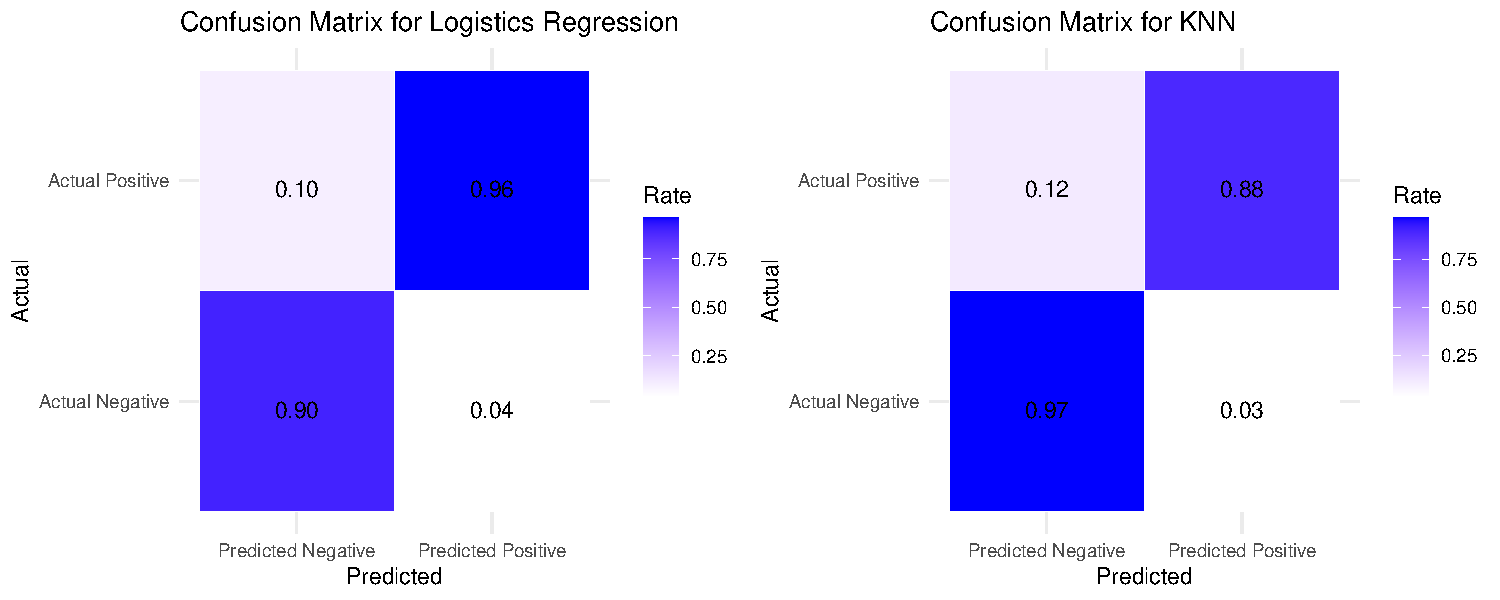
\includegraphics[width=\textwidth]{graphs/heatmaps.pdf}
		\caption{Logistic Regression heatmap and KNN hearmap.}
		\label{logistic}
	\end{figure}
	
	\section{Conclusion and Discussion}
	
	In summary, our project, "How You Distinguish People by Voice", revealed several findings about the correlation between various voice frequency data attributes and demographic factors including gender and age. 
	
	We have concluded the following key findings which answer the 4 questions above:
	1. Based on our analysis, the mean frequency between male and female voices has NO significant difference, as suggested by the statistical tests conducted.
	2. In fact, the male mean fundamental frequency is much higher than the female mean fundamental frequency. By conducting the Shapiro-Wilk Test and Wilcoxon Test, we obtain a relatively small p-value. Therefore, we reject the hypothesis where male mean fundamental frequency and female mean fundamental frequency are the same.
	3. As suggested from our analysis, males generally have a lower median frequency as compared to the female voice.
	4. Surprisingly from our analysis, there is enough evidence to support that the third quantile of males has greater values than that of females. However, upon examining the distribution graph, the difference is not very significant. On the other hand, there is enough evidence to support that the first quantile of males has smaller values than that of females.
	5. Generally, the features will have different mean values across different age groups.
	
	\newpage
	
	\bibliographystyle{plain} % or another style like apalike, abbrvnat, etc.
	\bibliography{references/ref} % assumes you have a references.bib file
	
	
	
	%%%%%%%%%%%%%%%%%%%%%%%%%%%%%%%%%%%%%%%%%%%%%%%%%%%%%%%%%%%%
	
	\newpage
	\appendix
	
	\section{Sample Code for the Project}
	\label{appendix:data_trans}
	
	\begin{figure}[ht]
		\centering
		\fbox{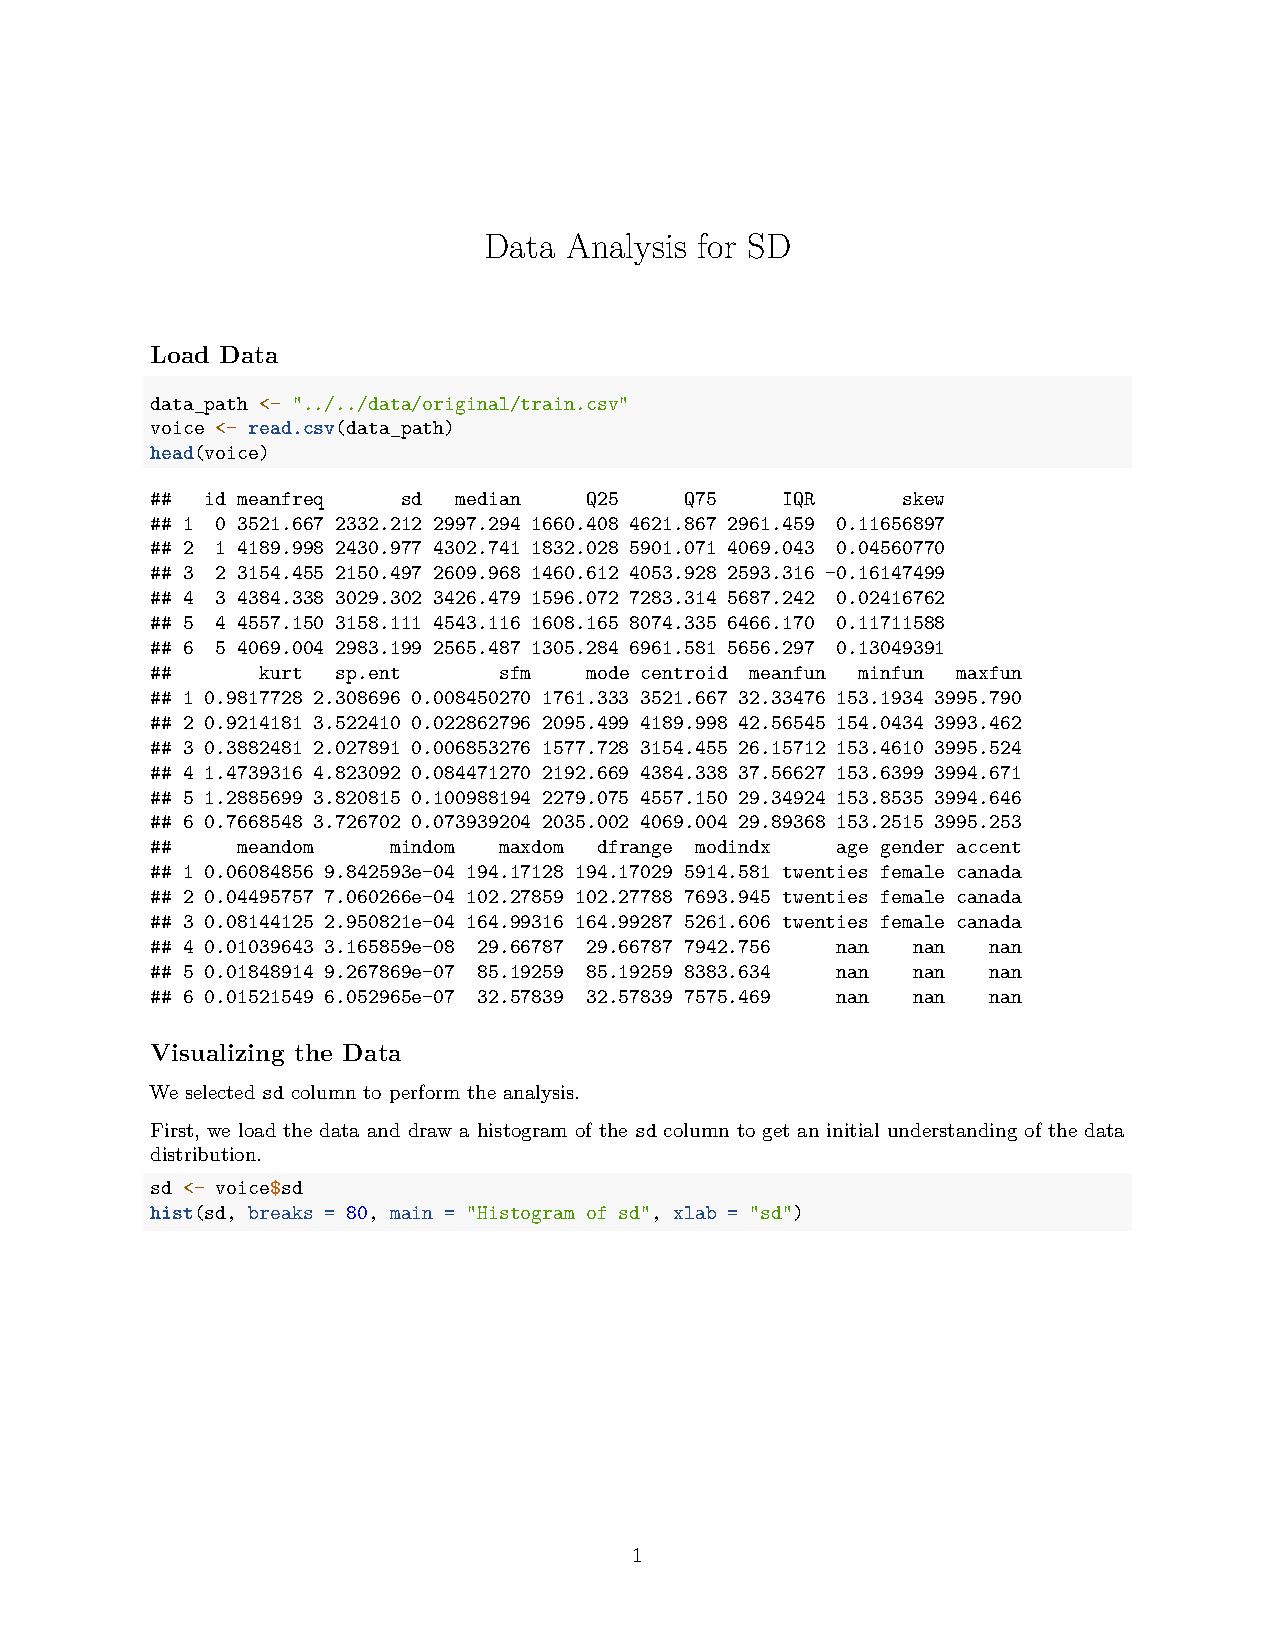
\includegraphics[page=1, width=\textwidth]{graphs/DataAnalysisSD.pdf}}
	\end{figure}
	\begin{figure}[ht]
		\centering
		\fbox{\includegraphics[page=2, width=\textwidth]{graphs/DataAnalysisSD.pdf}}
	\end{figure}
	\begin{figure}[ht]
		\centering
		\fbox{\includegraphics[page=3, width=\textwidth]{graphs/DataAnalysisSD.pdf}}
	\end{figure}
	\begin{figure}[ht]
		\centering
		\fbox{\includegraphics[page=4, width=\textwidth]{graphs/DataAnalysisSD.pdf}}
	\end{figure}
	\begin{figure}[ht]
		\centering
		\fbox{\includegraphics[page=5, width=\textwidth]{graphs/DataAnalysisSD.pdf}}
	\end{figure}
	
	\begin{figure}[ht]
		\centering
		\fbox{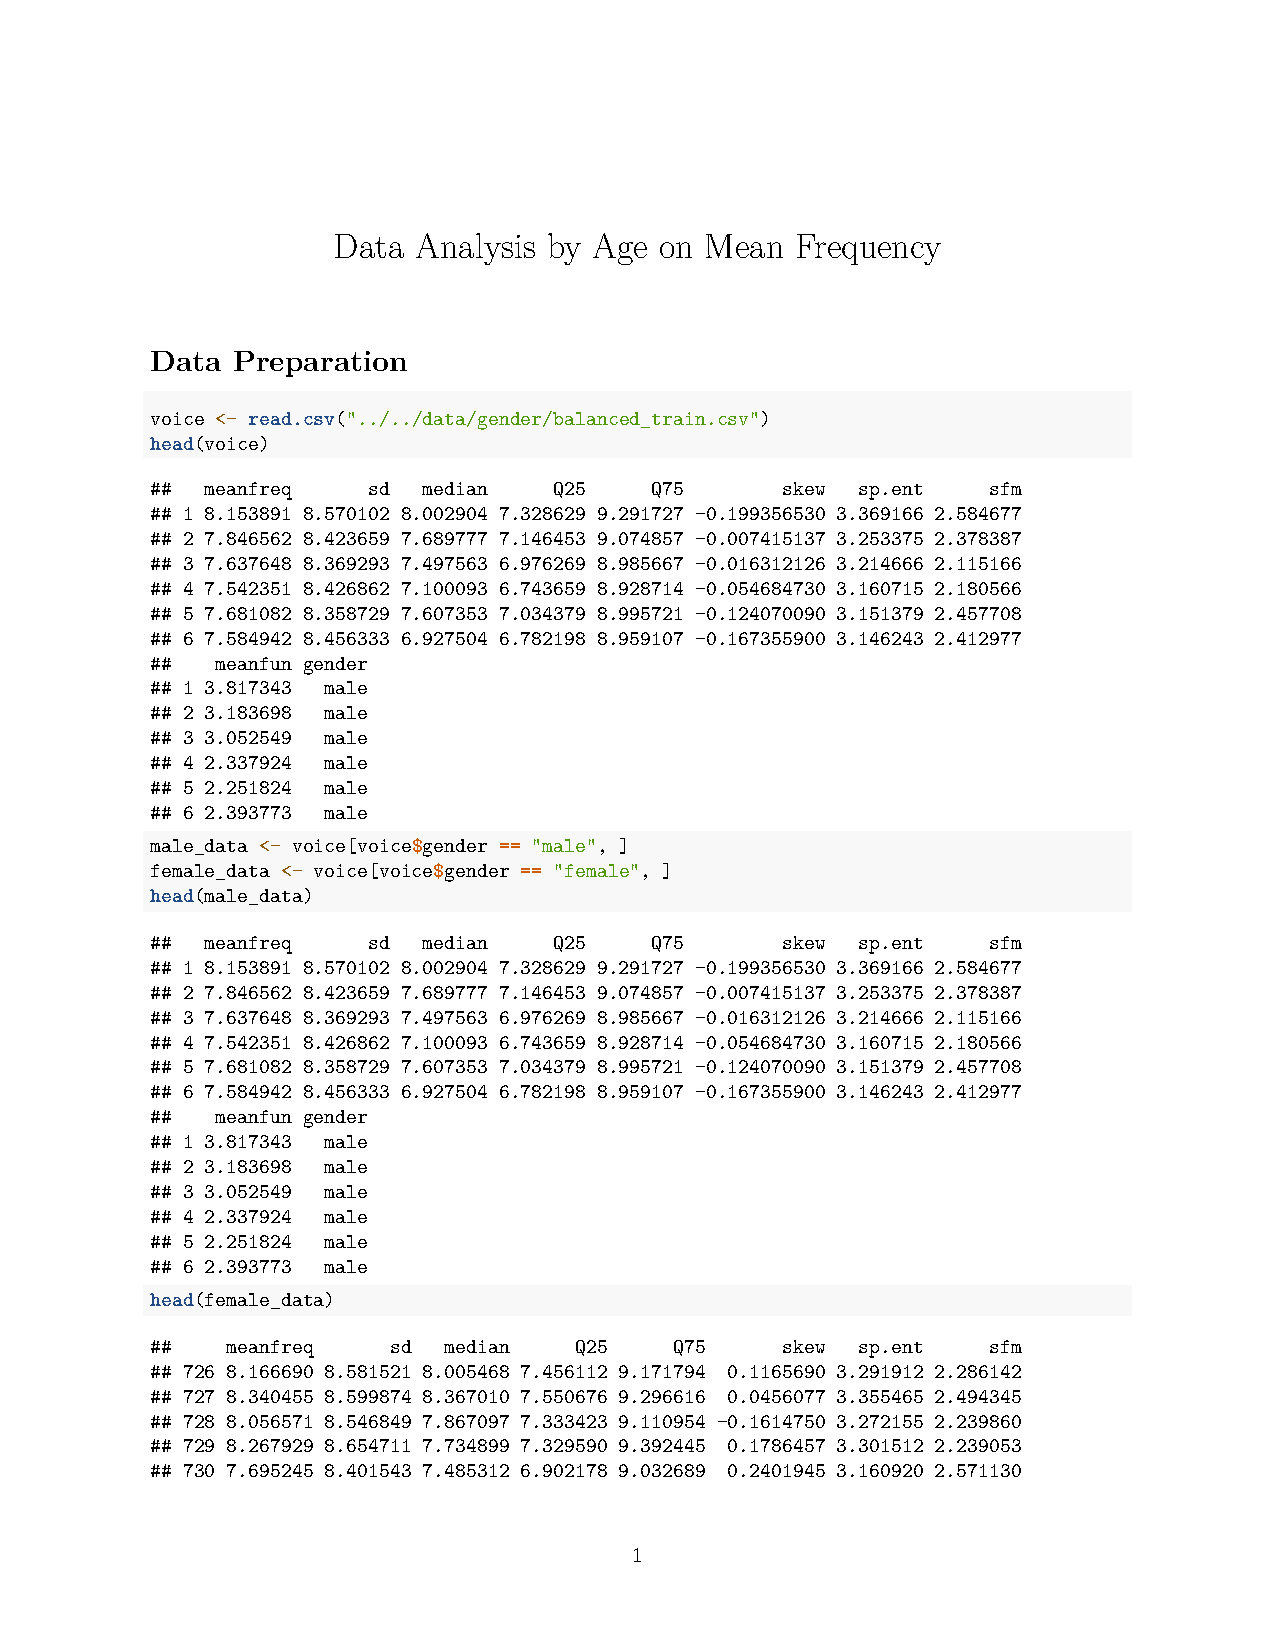
\includegraphics[page=1, width=\textwidth]{graphs/sample_analysis.pdf}}
	\end{figure}
	\begin{figure}[ht]
		\centering
		\fbox{\includegraphics[page=2, width=\textwidth]{graphs/sample_analysis.pdf}}
	\end{figure}
	\begin{figure}[ht]
		\centering
		\fbox{\includegraphics[page=3, width=\textwidth]{graphs/sample_analysis.pdf}}
	\end{figure}
	\begin{figure}[ht]
		\centering
		\fbox{\includegraphics[page=4, width=\textwidth]{graphs/sample_analysis.pdf}}
	\end{figure}
	\begin{figure}[ht]
		\centering
		\fbox{\includegraphics[page=5, width=\textwidth]{graphs/sample_analysis.pdf}}
	\end{figure}
	\begin{figure}[ht]
		\centering
		\fbox{\includegraphics[page=6, width=\textwidth]{graphs/sample_analysis.pdf}}
	\end{figure}
	\begin{figure}[ht]
		\centering
		\fbox{\includegraphics[page=7, width=\textwidth]{graphs/sample_analysis.pdf}}
	\end{figure}
	
	
	
	
\end{document}